\documentclass[12pt]{report}
\usepackage[utf8]{inputenc}
\usepackage[T1]{fontenc}
\usepackage{fancyhdr}
\usepackage{mathrsfs}
\usepackage{amssymb}
\usepackage{amsmath}
\usepackage{amsfonts}
\usepackage{caption}
\usepackage{tikz}
\usetikzlibrary{automata,arrows,positioning}
\usepackage{textcomp}
\usepackage{verbatim}
\usepackage{booktabs, tabularx}
\renewcommand\tabularxcolumn[1]{m{#1}}

\pagenumbering{arabic}
\pagestyle{fancy}
\rhead{NLP}
\renewcommand{\footrulewidth}{1pt}
\renewcommand{\arraystretch}{0.6}

\begin{document}
\title{Grundlagen zu Natural Language Processing und Analyse von GATE als NLP-Tool}
\author{Aaron Schul, Felix Ritter}
%\subtitle{Projektarbeit, Bearbeitungszeitraum Sommersemester 2018\\
%Fachhochschule Dortmund \\
%Fachbereich 4, Informatik}
\date{\today}
\maketitle

\newpage
\tableofcontents
\newpage
\listoftables
\listoffigures

\newpage
\section{Einleitung, später abstract}
Mit voranschreitender Globalisierung und immer größeren Mengen an übertragenen Informationen steigt auch die Menge an zu verarbeitender natürlicher Sprache. Während dies bisher manuell durch den Menschen geschah, kommt allmählich aufgrund der schieren Menge von Daten vor allem im unternehmerischen Kontext und im Internet die Notwendigkeit auf, die natürliche Sprache automatisiert durch Computer verarbeiten zu lassen.

Dies bezeichnet man als Natural Language Processing (kurz NLP). Es hilft dabei, Texte beispielsweise nach Schlagworten zu durchsuchen, strukturell zu analysieren, Muster zu erkennen und teilweise sogar die Bedeutung von Geschriebenem zu verstehen und diese Semantiken darzustellen.

Mit dem Aufkommen von NLP steigt auch das Interesse an NLP-Tools, also an Programmen, welche in der Lage sind, die für NLP notwendigen Funktionalitäten übersichtlich und praktikabel bereitzustellen. Eines der bekanntesten NLP-Tools ist das von der University Of Stanford entwickelte GATE, welches eine Vielzahl von Anwendungsbereichen im NLP abdeckt.

Das Ziel dieser Arbeit ist es, eine Anforderungsanalyse für solche Tools durchzuführen und diese dann mit dem GATE-Tool abzugleichen. Somit bietet sich die Möglichkeit GATE zu analysieren und daraufhin kriterienbasiert zu evaluieren. Funktionale wie nicht-funktionale Anforderungen werden definiert.

Zu diesem Zweck werden zunächst ausführlich die Grundlagen zu NLP und dessen Tools erläutert. Die Teilschritte der Textverarbeitung werden theoretisch wie praktisch anhand von Implementierungsbeispielen erläutert. Daraufhin können mit Hilfe von Use Cases Anforderungen an diese Tools erhoben werden, auf denen Analyse und Evaluation des GATE-Tools beruhen sollen. Abgeschlossen wird die Arbeit von einer kurzen Zusammenfassung der gewonnenen Erkenntnisse, gefolgt von einem Ausblick auf mögliche zukünftige Arbeiten und Entwicklungen für NLP-relevante Domänen. 
\newpage
\chapter{Einführung}
\section{Motivation und Herkunft}
Jeder Mensch kommuniziert alltäglich mit Anderen mithilfe von natürlicher Sprache. Dies ist bereits seit Jahrtausenden so, jedoch hat sich die Übertragung dieser Sprache mit der Zeit verändert und weiterentwickelt.\cite{wei89}

Damals lediglich von Mund zu Mund übertragen war der erste große Schritt die Entwicklung der Schrift. Mithilfe von Hieroglyphen, Alphabeten oder anderen Zeichen war man in nun in der Lage, natürliche Sprache über lange Zeit und/oder weite Strecken zu vermitteln. Dies erwies sich als sehr Vorteilhaft und so setzte sich die Entwicklung fort, bis man über das Morsen und das Telefon schließlich die elektronische Nachricht erfand. 
Im Rahmen der voranschreitenden Digitalisierung und Globalsierung steigt die Menge an übertragener natürlicher Sprache nach wie vor rasant an, sodass heute etwa E-Mails einen wesentlichen Bestandteil der Kommunikation ausmachen. Obgleich die Übertragung durch kabelgebundene oder drahtlose Kommunikation weitgehend automatisiert ist, erfolgt die Auswertung des Inhalts größtenteils manuell durch menschliche Empfänger.

Die Daten selbst sind jedoch inzwischen kaum noch nur durch den Menschen effizient zu verarbeiten, sodass man nach einer neuen Möglichkeit sucht, dem Menschen diese Arbeit zu erleichtern, oder sogar abzunehmen. Mit dieser Aufgabe beschäftigt sich NLP. Moderne Ansätze aus der Informatik, wie etwa Machine-Learning und dynamische Programmierung, sind dabei eng miteinander verwoben und sind aktuelle relevante Forschungsthemen.

\section{Hypothese}
Hypothese dieser Arbeit ist, dass NLP ein breit gefächertes Anwendungsgebiet der modernen Informatik ist. Die Abdeckung der Teilbereiche erfolgt durch verschiedene Werkzeuge, an welche besondere Anforderungen aus dem Requirements Engineering erhoben werden müssen.
(Hypothese dieser Arbeit ist, dass bestimmte algorithmische Verfahren besser oder schlechter für NLP geeignet sind, die im Laufe der Zeit entwickelt wurden.) Es stellt sich ferner die Frage, ob überhaupt ein ganzheitliches NLP unter Einbezug von Semantiken erforderlich ist und wenn ja, wie dann Wissen aus der Welt und um Sprache im Computer modelliert werden kann. 

\section{Methodik}
Verschiedene Ansätze für die Modellierung natürlicher Sprache werden zunächst erläutert, damit der Sinn und Zweck von NLP verdeutlicht wird. Die Teilschritte der Textverarbeitung werden für das Verständnis verschiedener Aspekte der Abläufe theoretisch wie praktisch mittels Implementierungsbeispielen erläutert. Anhand des Programms GATE wird überprüft, wie das Programm natürliche Sprache verarbeitet und inwiefern es unter Kriterien des Requirements-Engineering für die Praxis geeignet ist.

\section{Aufbau der Arbeit}
Beginnend mit einer kurzen Motivation und Historie wird zunächst in das Thema eingeführt. Bekannte Ansätze und Beispiele aus dem Alltag leiten in die Analyse über.

Für die Vermittlung von Wissen aus dem Bereich NLP werden zunächst ausführlich die Grundlagen zu NLP und dessen Aufgaben wie Tools erläutert. Daraufhin können mit Hilfe von Use-Cases Anforderungen an diese Tools erhoben werden, auf denen Analyse und Evaluation des GATE-Tools beruhen sollen. 

Abgeschlossen wird die Arbeit von einer kurzen Zusammenfassung der gewonnenen Erkenntnisse, gefolgt von einem Ausblick auf mögliche zukünftige Arbeiten und Entwicklungen für NLP-relevante Domänen. 

\chapter{Natural Language Processing}
\section{Grundlagen und thematische Einordnung}
Der folgende Abschnitt befasst sich mit den Grundlagen zu Natural Language Processing (im Folgenden kurz NLP). Dazu gehört neben dessen Herkunft bzw. Motivation eine inhaltliche Wissensgrundlage, welche für den weiteren Verlauf der Ausarbeitung relevant ist. 

\subsection{Definition}
NLP ist grob definiert als die automatische oder halb-automatische Verarbeitung von natürlicher Sprache. \cite{cop04} Manche schließen aus dieser Definition die Erfassung der Sprache aus, da diese nicht Teil der eigentlichen Verarbeitung ist. (Der Einfachheit halber wird im weiteren Verlauf davon ausgegangen, dass die Sprache als digitale Textdatei vorliegt, wenn nicht explizit anders angegeben. Es kann sich jedoch auch um gesprochenes Wort oder Gesten handeln)

NLP überschneidet sich mit vielen wichtigen Bereichen der Wissenschaft. Hauptsächlich sind dies Linguistik und Informatik, allerdings fließen auch Psychologie, Philosophie und Mathematik bzw. Logik stark mit ein. 

\subsection{Ziel und funktionale Einordnung}
Das Ziel von NLP ist die Extraktion von Informationen aus gegebenen Texten, also aus einem natürlichsprachlichen Input einen Wissensoutput über den Inhalt des Dokuments zu generieren. Dies wird mithilfe von NLP-Tools wie GATE umgesetzt.

Dazu ist, wie im nächsten Abschnitt beschrieben, die linguistische Analyse der Sprachstruktur der Dokumente in Teilschritten erforderlich. Auf Basis der syntaktischen Analyse kann dann eine semantische Analyse durch Einsatz sogenannter Ontologien (Sammlung von Wissen aus einer Domäne) erfolgen. Letztendlich kann somit tatsächlich Wissen über die Bedeutung aus dem Dokumenteninhalt gewonnen werden.

\subsection{Beispiele früher Entwicklungen}
Die Forschungsergebnisse des Linguisten Noam Chomsky seit den 1950er Jahren haben aufgezeigt, dass es grundsätzlich möglich ist, einge Aspekte der Regeln englischer Sprache zu formalisieren. In Kombination von beispielsweise Automaten und generativen Grammatiken (Abschnitt 2.4 und 2.6), die auch \textit{Chomsky-Hierarchie} genannt wird, wird verdeutlicht, wie diese automatisiert aufgefasst und nachvollzogen werden kann. Siehe dazu auch \cite{cho57}. Chomsky schaffte damit zum großen Teil die Grundlagen der Modelle heutiger Sprachanalyse-Tools.

Bereits in den 1960er Jahren versuchte man durch Sprachcomputer bzw. Chatbots wie \textit{ELIZA} \cite{wei66} die Mensch-Maschine-Kommunikation umzusetzen, indem die Textnachricht eines Benutzers automatisch durch einen Computer verarbeitet und eine plausible Antwort gegeben wurde, damals jedoch noch ohne echte Wissensbasis. Aus heutiger Sicht kann man ELIZA somit keine Möglichkeit zur "intelligenten" Kommunikation attestieren, da scheinbar der Sinn hinter den Nutzereingaben nicht gänzlich erfasst wird.

Heutige Entwicklungen im Bereich Sprachassistenzsysteme sind alltäglicher Begleiter jedes Smartphone-Nutzers geworden; sie analysieren die Spracheingaben mithilfe von NLP-Techniken bezüglich ihrer Bedeutung in Echtzeit über Clouds. \cite{hao14}

\subsection{NLP als Annäherung an natürlichsprachliche Probleme}
Bereits bei der Mensch-Mensch-Kommunikation sind  Verständigungsprobleme vorhandenen und treten unwillkürlich auf. Die Intention einer Aussage ist etwa nicht nur abhängig von dem, was tatsächlich gesagt wird, sondern auch etwa von Gestik, Mimik und der Situation, in der kommuniziert wird. Bei der Untersuchung von geschriebenem Text in natürlicher Sprache treten diese Betrachtungen jedoch in den Hintergrund, da der Inhalt im Vordergrund steht und mitunter die Situation des Autoren unklar oder irrelevant ist. Wissen aus der Domäne ist jedoch zwingend für das Verständnis spezifischer Fachbegriffe von Nöten, daher müssen auch automatische NLP-Tools diese einbeziehen können. Zudem gibt es oft Veränderungen der Bedeutung von Sprache die stark kontextabhängig sind, wie zum Beispiel Sarkasmus oder Ironie. Auch verändern Worte im Laufe der Zeit ihre Bedeutung oder durch Rechtschreibreformen ihr Aussehen. Hier soll nicht weiter auf Aspekte der Kommunikationswissenschaften eingegangen werden, jedoch ist beispielsweise die Ambiguität einer Aussage ganz alltäglich und hat gleichsam verschiedene Auswirkungen. Solche Mehrdeutigkeiten können syntaktische und semantische Fehlinterpretationen verursachen. \cite{wei89}

Wo sich Menschen dabei im Zweifel auf Erfahrungen und spezifische Fachkenntnisse verlassen oder bei ihrem Kommunikationspartner nachfragen können, müssen sich Computer allein auf die vorliegenden Dokumente in Schriftform verlassen; sie wissen nichts über den Kontext des Dokuments. Wie später gezeigt wird, kann jedoch etwa Fachwissen durch domänenspezifische Wissensbasen (siehe Abschnitt 3.8.2) simuliert werden. 

Die Frage nach einer intelligenten, algorithmen- und / oder wissensbasierten Auswertung durch Computer stellt sich im Angesicht der aufgezeigten Besonderheiten natürlicher Sprache. Es gilt also, für NLP nicht nur die Probleme zu lösen, die generell mit präziser Automatisierung verbunden sind, sondern zusätzlich so zuverlässig wie möglich die oben genannten und der Sprache inhärenten Komplikationen zu bewältigen. 
Bereits einfache Anfragen können computergestützte Frage-Antwort-Systeme wie SQL-Datenbanken an ihre Grenzen bringen, wie die verschiedenen Formen von Mehrdeutigkeit zeigen können:

Schon das Wort \textit{überblicken} kann das Übersehen von etwas, ebenso wie das im Blick haben (Gegenteil) bedeuten.

Der Satz \textit{"Die Betrachtung des Studenten"} kann etwa als Student, der (etwas) betrachtet, oder als ein Student, der (von jemand anderem) betrachtet wird, verstanden werden. Sätze mit solch einem Satzbau (bestehend aus nominalisiertem Verb, Bezugswort und Substantiv) verursachen unwillkürlich zwei mögliche Deutungen aufgrund der unklaren Syntax.

Die Frage \textit{"Verkaufen Sie Handys und Computer von Samsung?"} kann als Frage nach allgemeinen Handys und nur Computern, spezifisch von Samsung oder nach Handys und Computern gleichermaßen nur von Samsung verstanden werden. Auch hier entsteht Unklarheit durch zwei mögliche Bezüge des einschränkenden Relativsatzes. Ob eine Aufzählung oder ein Unterschied (zwischen \textit{von Samsung} und \textit{nicht von Samsung} gemacht wird, ist syntaktisch unklar.)

\textit{"Wie schnell ist der Bus?"} und \textit{"Wie schnell ist der Bus da?"} mögen zunächst ähnlich aussehen, fragen jedoch unterschiedlichen Inhalt ab und haben nichts miteinander zu tun. Außerdem könnte der zweite Satz kontextabhängig etwa nach der Fahrzeit bis zum Ziel oder nach der Ankunftszeit, an der man einsteigen kann, fragen. Die vage Formulierung von Sätzen stellt bei der Frage nach deren Bedeutung eine Herausforderung dar, durch Untersuchung des Kontextes der Frage kann hier jedoch meist recht treffsicher geantwortet werden.

Abgesehen von diesen syntaktischen Uneindeutigkeiten muss NLP auch Hürden der inhaltlichen Mehrdeutigkeit bzw. Semantik bewältigen. Aktuell beschäftigt man sich zum Beispiel mit der Aufgabe zu erkennen, ob ein Kommentar zu einem Video der Webseite \textit{Youtube} eher positiv oder eher negativ gesinnt ist. Was hier für den Menschen schon beim ersten Lesen sofort erkennbar wird, stellt für den Computer ein ernstzunehmendes Problem dar. Tonalität und Stimmung des Kommentars, der unter einem Video als Reaktion entsteht, sind mitunter nicht direkt aus dem audiovisuellen Eindruck aus dem Video ersichtlich. (?)
Solche scheinabr simplen Probleme sind für den Menschen recht einfach zu lösen. Wie oben erwähnt existiert NLP bereits seit ca. Mitte des 20. Jahrhunderts, jedoch ist die Behandlung natürlichsprachlicher Probleme auch heute noch problematisch in der Implementierung. Wenn Systeme die oben genannte Beispiele nicht explizit ausschließen, muss die Verarbeitungslogik besondere Rücksicht auf Uneindeutigkeiten nehmen.

\subsection{Konzepte aus der Logik für NLP-Anwendungen}
Weit vor der Implementierung von NLP mittels Tools haben sich Logiker und Experten aus der theoretischen Informatik mit der Frage beschäftigt, wie man Sprache und Ereignisse aus der echten Welt in logischen Ausdrücken formalisieren kann. Ausgehend von der klassischen Aussagenlogik wurde mit der parametrisierten $\in_T$-Logik nach Zeitz \cite{ze00} ein Ansatz geschaffen, der eine Darstellung von Semantik in propositionalen Logiken ermöglicht. Nach Martin-Löf \cite{ml96} beschreibt eine Proposition den "Gedanken oder Sachverhalt eines formalen Ausdrucks", die dann in einer $\in_T$-Logik dargestellt werden kann und somit einen Sachverhalt als Symbol abbildet. Ziel ist es, tatsächlich Bedeutungen in Form von Propositionen mittels Formeln aus Symbolen der Logik darzustellen. Abstrakt betrachtet kann man sich mit propositionalen Logiken einer Abbildung von Wissen aus der tatsächlichen Welt annähern. 

Die klassische Aussagenlogik kann etwa Wissen mittels ihrer Symbole abbilden, indem Sie Formeln aus diesen Symbolen bildet. Jedem Symbol ist dabei eine Aussage zugeordnet, dass dann in einer Formel als Variable auftaucht. Problematisch ist jedoch, dass solch eine Logik bei der Deutung auf reine Wahrheitswerte dieser Formeln beschränkt ist, indem die Symbole logisch wahr oder falsch belegt werden. Eine explizitere, semantische Deutung der Formeln ist jedoch erforderlich, um tatsächlich metasprachliche Aussagen in einer Logik zu formulieren. 

$\in_T$-Logiken erweitern zugrundeliegende Logiken deshalb dahingehend, dass nicht nur die logische Korrektheit (die Formel ist syntaktisch korrekt) überprüft wird, womit auch Mehrdeutigkeiten und Missverständnisse akzeptiert würden. Die Bedeutung hinter den Symbolen, die Propositionen, werden erfasst. $\in_T$-Logiken können also auch die semantische Bedeutung einer Aussage überprüfen, indem sie entsprechende Ausdrucksmittel enthält:
\begin{enumerate}
\item propositionale Gleichheit (zwei Aussagen sind gleichbedeutend)
\item Prädikate für wahr und falsch (Semantik, kein logischer Wahrheitswert)
\item Quantifizierung über Propositionen (Umformulierung als messbare Eigenschaft)
\end{enumerate}
Mittels $\in_T$-Logiken kann man sich etwa der Behandlung von natürlichsprachigen Problemen, wie beispielsweise Antinomien, annähern, da diese eine logische Betrachtung und Deutung ermöglichen. Sie stellt daher eine Abstraktion und theoretische Grundlage der Lösungsansätze für Probleme aus Mehrdeutigkeiten und Semantik dar, die unter 3.8 und 3.9 praktisch beschrieben werden.

\section{Linguistische Analyse}
Der folgende Abschnitt beschäftigt sich mit der Analyse der sprachlichen Struktur eines Dokumentes. Am Anfang von NLP steht die linguistische Analyse des Textes etwa bezüglich Satzstruktur und Differenzierung von Wörtern aus der Sprache und Eigennamen. Das Ziel ist die sogenannte \textit{Annotation} der Textbausteine bezüglich ihrer Bedeutung. Übergreifende Sachzusammenhänge anhand der Relationen von Wörtern sollen dargestellt werden.

NLP kann, wie später in dieser Arbeit beschrieben, als Umsetzung vierer wesentlicher Teilbereichen aus der Linguistik verstanden werden. Begonnen bei der einfachen Wortanalyse, werden später Bedeutungen und Verknüpfungen der Aussage aus Sätzen oder Wörtern auf die reale Welt analysiert. Die Linguistik befasst sich seit jeher mit der Untersuchung von natürlicher Sprache im Hinblick auf die dahinter liegenden Konstrukte. Die folgenden Teilbereiche, die daraus bekannt sind, sind bei der natürlichsprachigen Analyse identifiziert worden:

\begin{enumerate}
\item
Morphologische Analyse - Die Zerlegung von Wörtern bezüglich ihrer Struktur. Die Komposition aus Präfix, Wortstamm und Suffix von Wörtern wird erkannt, um Fall, Tempus, Numerus etc. des Wortes zu bestimmen. Im Englischen zeigt so die Endung -ed bei Verben die Vergangenheitsform an. Dabei ist zu beachten, dass Mehrdeutigkeiten entstehen können.
\item
Syntax - Aufbau von Sätzen durch einzelne Wörter. Jede Sprache besitzt syntaktische Regelungen bezüglich der auftauchenden Wörter; im Deutschen folgt etwa auf einen Artikel irgendwann ein Substantiv oder bestimmte Signalwörter geben Satztyp und Tempus an. Auf Basis dieses Wissens können formale und strukturelle Analysen der Textbestandteile erfolgen.
\item
Semantiken - Die Identifikation der Bedeutung von einzelnen Sätzen und Wörtern. Die Semantik eines Textabschnittes wird häufig als "Logik" bezeichnet und fragt nach dessen Bedeutung bzw. Thema. Semantische Deutungen können anhand von Kompositionen einzelner Wörter und Sätzen auf Basis der semantischen Analyse erkannt werden.
\item
Kontext - Darstellung von Sachzusammenhängen aus der Vereinigung von ähnlichen Bedeutungen. Textbausteine, die sich mit dem gleichen Thema beschäftigen, werden dem gleichen Sachzusammenhang zugeordnet und als Teil dessen annotiert.
\end{enumerate}

NLP spaltet bei der Analyse diese Sprachbestandteile aus der Linguistik weiter in Teilbereiche auf und ordnet diese Aufgaben in der Implementierung Programmbausteinen zu.

\subsection{Allgemeine NLP Architektur}
Die Verarbeitung eines Dokumentes mittels NLP erfolgt nacheinander in einzelnen Schritten, die jeweils einen Bereich oder Teilbereich der Linguistik des Textes abbilden. Die Analyse erfolgt dabei nacheinander und wird immer feingranularer, begonnen bei einfachen grammatikalischen Analysen bis hin zu komplexen Wissensbasierten verfahren. Die folgenden Schritte stellen laut \cite{cop04} eine typische komponentenweise Architektur dar. Es ist anzumerken, dass auch mehrere Schritte gemeinsam in einem Schritt durchgeführt oder gar ganz entfallen können, abhängig von der Umsetzung anderer Stufen:

\begin{enumerate}
\item
Input Processing - Erkennung der Dokumentensprache und Normalisierung des Textes. Im ersten Schritt geht es um das korrekte Format des Eingabedokumentes für die Verarbeitung. Dieser Vorgang stellt jedoch noch keine Analyse dar, sondern dient lediglich der Vorbereitung.
\item
Morphologische Analyse - Die meisten Sprachen sind im Bezug auf ihre Grammatik und syntaktische Struktur der Wörter in Systemen abgeschlossen, etwa durch Modellierung mittels Automaten zur Erzeugung der Worte. Auch können Vokabeln in Wörterbüchern/Lexika gesammelt und Regeln auf ihnen formuliert und gespeichert werden.
\item
Part-of-Speech-Tagging - Die einzelnen Wörter eines Satzes werden im Hinblick auf den Sach- oder Satzzusammenhang, wie auch auf die Stellung der Stellung im Satz hin analysiert. Basierend auf Kontext und/oder Erfahrungswerten bzw. Heuristiken können die Wörter korrekt erfasst und deren Fall getaggt werden. Subjekte, Prädikate usw. werden identifiziert. Dazu ist eine Wissensbasis mit Trainingsdaten und die Einordnung des Kontextes darin von Nöten.
\item
Parsing - Die Ergebnisse der  der vorherigen Schritte werden weiter verarbeitet und in ein standardisiertes Format gebracht. Syntaktische Zusammenhänge, wie etwa das Zusammenfassen von Wörtern zu einer gemeinsamen Bedeutungsphrase und das Zuordnen von Verben zu einem Nomen können nach dem Parsing dargestellt werden.
\item
Disambiguation - Die Entfernung von Mehrdeutigkeiten auf Basis der Ergebnisse des Parsings stellt einen entscheidenden Schritt für die semantischen Analysen dar. Nur wenn die Aussage und der Kontext eines Satzes klar erkennbar sind, kann dessen Semantik gezielt abgeleitet werden.
\item
Context Module - Textbausteine, deren Interpretation semantisch auf dem Kontext anderer Sätze oder Wörtern beruhen, können erfasst werden. Bei Anaphern ist etwa das Verständnis des aktuellen Kontext abhängig von einer vorherigen Deutung.
\item
Text Planning - Die Sachzusammenhänge und Semantiken, die aus dem zugrundeliegenden Text extrahiert wurden, werden für die Darstellung im fertigen Text definiert. Es wird festgelegt, welche der Bedeutungen qualitativ übertragen und vermittelt werden sollen. Die Reihenfolge und Umfang der behandelten Themen wird geschätzt und definiert.
\item
Tactical Generation - Die Bedeutungen werden in Form konkreter Zeichenketten generiert, die die gewünschte Bedeutung enthalten. Diese Textbausteine basieren häufig direkt auf den Ergebnissen des vorherigen Parsings, da dort schon Bedeutungen zusammengefasst werden können. Der quantitative Teil des Textes wird erzeugt.
\item
Morpholigical Generation - Die erzeugten Sätze werden morphologisch an die Rahmenbedingungen der verwendeten Sprache angepasst. Grammatiken und Regeln der Satzkonstruktion werden auf die erzeugten Wörter angewendet, sodass ein lesbarer und nachvollziehbarer Text entsteht.
\item
Output Processing - Der Text wird nun, nachdem dieser inhaltlich nun komplett erzeugt vorliegt, an das Design und Format des jeweiligen Einsatzzwecks angepasst. Sollte Text, anders als in dieser Arbeit der Einfachheit halber angenommen, nicht als geschriebenes Wort ohne besondere Formatierung vorliegen, kann dieser einem Formatter zur Designanpassung übergeben werden. Ferner kann etwa mihilfe von Text-to-Speech eine Audioausgabe erfolgen. 
\end{enumerate}

\section{Morpholoie in NLP}
Der folgende Abschnitt befasst sich genauer mit der morphologischen Analyse von Wörtern und den dazu verwendeten Zustandswandlern. Da in der englischen Sprachanalyse bereits die meisten Fortschritte erzielt wurden und sie verhältnismäßig wenig komplex im Vergleich zu anderen Sprachen ist, werden im Folgenden viele der Beispiele auf Englisch behandelt. (? vielleicht trennen)

Wie bereits erwähnt, befasst sich die Morphologie mit der Struktur, Zusammensetzung und Korrektheit einzelner Wörter. Jedes Wort der englischen Sprache besteht aus mindestens einem Wortstamm und beliebig vielen Affixen. Affixe sind unterteilt in Präfixe und Suffixe, abhängig davon, ob sie vor oder hinter dem Wortstamm auftauchen. Es gibt auch Affixe, welche in der Mitte des Wortes eingeordnet werden. Diese existieren jedoch nicht in der englischen Sprache und sind daher künftig zu vernachlässigen. (? Reihenfolge)

Man betrachte beispielsweise das Wort \textit{"believe"} von dem englischen Verb \textit{"to believe"} (zu Deutsch: "glauben"). Hängt man das Suffix \textit{"-able"} an, so erhält man das Adjektiv \textit{"believable" ("glaubhaft")}. Fügt man nun das Präfix \textit{"un-"} hinzu erhält man die Negation \textit{"unbelievable" ("unglaubhaft")}. Die morphologische Analyse erkennt dies nicht nur als ein Wort, sondern als Präfix-Stamm-Suffix-Konstrukt.

Es wird zwischen ableitender und flexionaler Morphologie unterschieden, wobei die Abgrenzung jedoch nicht ganz eindeutig ist. Affixe wie \textit{"anti-"}, \textit{"re-"} und das oben verwendete \textit{"un-"} gelten als ableitend und können mehrfach und sogar rekursiv zu Stämmen auftauchen. Sie fügen dem Stamm in der Regel eine Zusatzinformation hinzu, wie z.B. Negation. Es kann auch, wie in dem Beispiel oben demonstriert, zur Änderung der Wortart kommen. Flexionale Affixe werden normalerweise aufgrund grammatikalischer Regeln wie Pluralisierung hinzugefügt. Hierzu gehören das Plural-"-s" und die Endung \textit{"-ed"} in der Vergangenheitsform. 

Die morphologische Analyse ist üblicherweise eine Vorarbeit für das Parsen von Texten, welches in Abschnitt 2.6 genauer beschrieben ist. Dafür sind jedoch genauere syntaktische und semantische Informationen nötig. So würde beispielsweise das Wort "fishing" eindeutig durch die "-ing"-Endung als Verb im Partizip Präsens erkannt, während bei dem Wort "fish" eine Mehrdeutigkeit zwischen dem Verb "fischen" und dem Substantiv "Fisch" die Verarbeitung verkompliziert. Dies wird durch das sogenannte Part-of-Speech-Tagging gelöst, welches in Abschnitt 2.5 behandelt wird.

\subsection{Lexika in der Morphologie}
Für eine präzise morphologische Analyse bedarf es 3 verschiedener Lexika, um mögliche Interpretationen zu speichern:

\begin{enumerate}
\item Liste von Affixen (zusammen mit den Informationen, die damit verbunden sind, z.B. Negation \tt "un-"\rm)
\item Liste von unregelmäßigen Wörtern (zusammen mit den Informationen, die damit verbunden sind, z.B. \tt "went":simple past"(to) go"\rm)
\item Liste von Wortstämmen (zusammen mit syntaktischer Kategorie, z.B. \tt "believe":verb\rm)
\end{enumerate}

Die Affix-Liste könnte in einen Präfix- und einen Suffix-Teil getrennt werden, welche jeweils das Affix und die oben beschriebenen Informationen als formatierten Text enthalten, in etwa wie folgt (Suffix-Teil):
\\
\tt
ed PAST\_VERB\\
ed PSP\_VERB\\
s PLURAL\_NOUN\\
\rm
\textit{PAST\_VERB}, \textit{PSP\_VERB} und \textit{PLURAL\_NOUN} beinhalten die durch den jeweiligen Suffix hinzugefügten Informationen über das Wort. 

Ähnlich verhält es sich mit der Auflistung der unregelmäßigen Formen. Das Affix wird hier durch die unregelmäßige Form ersetzt und es ist zu beachten, dass es nötig ist, zu den in 1. vorhandenen Informationen auch den Referenz-Stamm anzugeben, in etwa wie folgt:
\\
\tt
began PAST\_VERB begin\\
begun PSP\_VERB begin\\
\rm
\textit{"Began"} und \textit{"begun"} sind hier jeweils die "PAST\_VERB"- und "PSP\_VERB" (past participle)-Form des Referenzstammes \textit{"begin"}.

Um unnötige Fehler zu vermeiden ist es ratsam, zusätzlich ein Lexikon mit Wortstämmen zu verwenden, welches die Wortstämme und eine grammatikalische Einordnung beinhaltet. Dies hat hauptsächlich zwei Gründe: 

\begin{enumerate}
\item Die Form im Zusammenhang mit vielen syntaktischen (siehe Abschnitt 2.5) und morphologischen Regeln ist wichtig. Die \textit{"-able"}-Anhangsregel kann beispielsweise nur bei Verben verwendet werden, die dann ein Adjektiv darstellen (diese Eigenschaft würde in der Affix-Liste beschrieben).
\item Mögliche Wortstämme überprüfen zu können ist wichtig, da somit viele Mehrdeutigkeiten ausgeschlossen werden können. So könnte "bus" z.B. als "bu$\textasciicircum$s" (Plural von "bu") interpretiert werden. Dies ist jedoch nicht möglich, wenn kein Eintrag zu dem Wortstamm "bu" existiert. 
\end{enumerate}

\subsection{Buchstabierregeln mit endlichen Zustandswandlern}
In der Morphologie gibt es eine Vielzahl von Regeln, die bei der Unterteilung, Interpretation und Zusammensetzung von Wörtern zu beachten sind. Wenn man das "believe"-Beispiel aus Abschnitt 2.4 erneut betrachtet, fällt auf, dass bei dem hinzufügen des Suffixes "-able" der letzte Buchstabe des Wortstammes entfällt. Dies ist natürlich kein Tippfehler, sondern beruht auf einer der besagten Regeln. Die oben verwendete Regel lässt sich wie folgt darstellen:
\tt
\begin{center}
e $\rightarrow \varepsilon \textasciicircum \_$able
\end{center}
\rm
Das \textit{e} ist in dem Falle der in Frage stehende Buchstabe, welcher, symbolisiert durch den Pfeil, in das $\varepsilon$ (das leere Wort) gewandelt wird, falls ein Affix angehängt wird ($\textasciicircum$) und es an dieser Stelle ($\_$) steht, also vor dem \textit{"-able"}.

Solche Regeln lassen sich zu morphologischen Zwecken gut mit endlichen Zustandswandlern (finite state transducers) realisieren, was im Folgenden demonstriert werden soll.

\subsection{Endliche Zustandswandler zur Umsetzung von morphologischen Regeln}
Ein endlicher Zustandswandler ist ein Graph aus einer endlichen Anzahl von Knoten (Zuständen), welche durch Kanten verbunden sind. Knoten sind unterteilt in einen Start-Knoten, eine beliebige Anzahl an normalen Knoten und mindestens einen Ziel-Knoten. Der Start-Knoten als Input das zu verarbeitende Wort, welches nun in eine Abbildung der Aufbaustruktur des Wortes übertragen werden soll. Das Erreichen eines Ziel-Knotens heißt, dass das Wort korrekt ist und akzeptiert werden kann. Die Kanten repräsentieren die Abbildung einer Zeichenkette auf eine andere. Dies funktioniert bidirektional, wodurch sie sowohl zum Erstellen, als auch zum Auflösen von Wörtern verwendetet werden können \cite{cop04}. Die folgende Abbildung zeigt den eindlichen Zustandswandler, der die Umsetzung der besagten "able"-Anhangs-Regel ermöglicht:
\\

\begin{figure}
\begin{center}
\begin{tikzpicture}
\node[accepting] (a) at (0,0)  [circle, draw, minimum size=10ex] {1};
\node (b) at (4,0)  [circle, draw, minimum size=10ex] {2};
\node (c) at (4,-4) [circle, draw, minimum size=10ex] {3};
\node[accepting] (d) at (0,-4) [circle, draw, minimum size=10ex] {4};
\draw[thick, ->] (a) to [bend left] node[midway, above] {$\varepsilon$ : e} (b);
\draw[thick, ->] (a) to [loop above] node[midway, above] {other : other} (a);
%\draw[thick, ->] (b) to [bend left] node[midway, below] {e : $\varepsilon$} (a);
\draw[thick, ->] (b) to [bend left] node[midway, right] {$\varepsilon : \textasciicircum$} (c);
\draw[thick, ->] (c) to [bend left] node[midway, below] {able:able} (d);
\end{tikzpicture}
\caption{Nicht-deterministischer Zustandswandler der able-Regel}
\end{center}
\end{figure}


Der oben abgebildete Zustandswandler ist in der Lage die beschriebene Regel umzusetzen wie folgt: In Zustand 1 erfolgt der Input des eingelesenen Wortes, also in diesem Falle \textit{"believable"}. Über die Schleife mit \textit{"other:other"} ist die Abbildung aller nicht speziell angegebenen Zeichenfolgen auf sich selbst beschrieben. Es kann jederzeit das leere Wort auf ein \textit{"e"} Übertragen werden, dies geschieht jedoch nur, falls auch ein "-able" folgt. In dem Fall wird zuvor noch aus dem leeren Wort ein Affix-Zeichen ($\textasciicircum$) generiert (Es ist anzumerken, dass der Zustandswandler nicht deterministisch ist, sich jedoch über die Potenzmengenkonstruktion immer ein äquivalenter deterministischer Zustandswandler erstellen ließe). So wird also das Wort "believable" durch diesen Automaten als "believe$\textasciicircum$able" Interpretiert, und somit das "able"-Affix erkannt. Andersherum ließe sich aus dem Wortaufbau "believe$\textasciicircum$able" das korrekte Wort "believable" generieren.

Üblicherweise werden für jede Regel eigene Zustandswandler erstellt, welche dann bei der Verarbeitung von Wörtern parallel ablaufen. Dies ist gut für die Performanz, birgt allerdings Probleme. Wenn man mit komplexen Wörtern arbeitet, bei denen mehrere Regeln gleichzeitig anzuwenden sind, können verschiedene valide Ergebnisse erzielt werden. So wäre es etwa problematisch zwischen den Wörtern "un$\textasciicircum$ion$\textasciicircum$ise$\textasciicircum$ed" (Chemie) und "union$\textasciicircum$ise$\textasciicircum$ed" (gewerkschaftlich organisiert) zu unterscheiden. 

\section{Part-of-speech tagging und Wortvorhersage}
Dieses Kapitel befasst sich mit der Transformation von Ergebnissen der morphologischen Analyse einzelner Wörter in eine sinnvolle Kategorisierung der Wörter im Sachzusammenhang aus mehreren Wörtern. Part-of-speech tagging klassifiziert einzelne Worte eines Textes so, dass erfasst wird, welche Rolle sie im Satz spielen. Die einzelnen Wörter des Textes werden im Englischen bezüglich ihrer grammatikalischen Funktion und Anzahl markiert (\textit{annotiert}). Die Identifikation muss so erfolgen, dass sie den Kontext des Satzes erfasst, also insgesamt Sinn ergibt. Diese Kennzeichnung geht über die Analyse einzelner Wörter hinaus; Sie erfasst auch die Syntax umgebender Wörter eines Satzes. 

Im Deutschen ist es etwa recht wahrscheinlich, dass auf ein Nomen am Satzanfang als nächstes Wort ein Verb folgt, da dies einen typischen Satzbau darstellt. Ein part-of-speech Tagger sollte daher beispielsweise im Satz \textit{"Ich fahre Fahrrad."} korrekt das "Ich" als Subjekt, das "fahre" als Prädikat und das "Fahrrad" als Akkusativobjekt darstellen; Die isolierte Betrachtung von \textit{"Fahrrad"} ließe aber auch die Kategorisierung als Subjekt zu, da sich die zwei Möglichkeiten bezüglich der Morphologie nicht unterscheiden. Diese Mehrdeutigkeit einzelner Worte im Satz wird durch Analyse des syntaktischen Kontextes eliminiert, sodass POS tagging eine Eindeutigkeit der syntaktischen Deutung erzielt.

Solche Regelmäßigkeiten werden in Form von sogenannten \textit{corpora} geliefert; sie stellen Trainingsdaten in Form von tatsächlicher Sprache dar. Im Englischen wird etwa häufig die Zeitung The Wall Street Journal genutzt, um die Repräsentation bestimmter Satzstrukturen und Wortfolgen statistisch zu erfassen. Eine Implementierung auf dieser Basis beschreiben etwa Toutanova et al. \cite{tou03}. 
\cite{tou03} taggt zu etwa 97,24\% korrekt, der Vorschlag aus \cite{she07} erreicht auf Basis einer bidirektionalen Analyse und Machine-Learning sogar 97,33\%.
 Alternativ können auch standardisierte Corpora wie der Lancaster-Oslo-Bergen Corpus verwendet werden, der etwa eine Million Wörter in Sprache enthält. Corpora sind etwa für NLP auf Basis von Machine-Learning-Algorithmen erforderlich, können darüber hinaus aber auch etwa zur Rechtschreibprüfung oder Textunterteilung benutzt werden. Die meisten Textverarbeitungsprogramme können heutzutage etwa erkennen, wenn sich syntaktische Fehler in einem Satz ereignen (Kommasetzung, falscher Kasus, etc.). Es ist anzumerken, dass part-of-speech tagging nicht unbedingt vorher annotierter Texte bedarf, aber ohne diese eine syntaktische Einordnung ungleich schwerer fällt und die Fehlerquote massiv steigt. Mehrdeutigkeiten aus der Syntax heraus können somit nicht aufgeschlüsselt werden.

Die Anwendung eines Corpus auf ein natürlichsprachliches Dokument ermöglicht sogleich auch eine Vorhersage der nächsten Wörter bzw. Sprachbausteine, nachdem schon ein Teilsatz gelesen wurde. Diese \textit{prediction} kann auf Basis bekannter Regelmäßigkeiten also schon vor der Wortanalyse recht genau die nächste grammatikalische Komponente bzw. den Worttyp vorhersagen.

\subsection{N-gram Modelle zur Sprachvorhersage und -modellierung}
Auf Basis der vorliegenden Corpora existieren eine Vielzahl an Regeln bezüglich des Satzbaus und bekannnter Folgen von Worttypen, wenn ein neues Dokument annotiert werden soll. Zur Veranschaulichung einer möglichen Annotation soll in diesem Abschnitt die Notation \cite{clw7} für Annotationen genutzt werden.

Bei erneuter Betrachtung des obigen Beispiels \textit{"Ich fahre Fahrrad."} könnte dieses, wenn dieser Satz als minimaler Corpus vorliegt, neben der Regel Subjekt-Prädikat-Objekt eines Satzbaus auch beinhalten, dass der Punkt ein Satzende markiert und das Substantive und Satzanfänge mit einem Großbuchstaben beginnen ("Fahrrad" ist gemäß der Morphologie ein Nomen und ist groß geschrieben). Sprachvorhersage nutzt diese bekannten Regeln und würde etwa aus der obigen Regel herleiten, das, wenn ein Verb gelesen wurde, darauf immer ein Substantiv bzw. das Satzobjekt folgt. POS-Tagging macht sich diese Beobachtungen durch Berechnung von Wahrscheinlichkeiten bei der Annotation von Wortfolgen zunutze. 

Kontextfreie Betrachtung einzelner Wörter, also ohne andere Taggings mit einzubeziehen, wird als Unigramm bezeichnet. Dabei werden jedoch Regeln über den Zusammenhang von Wortketten vollständig ignoriert und das Ergebnis ist ähnlich dem der morphologischen Analyse. Vorhersage-Systeme, die sich der Annotierung des vorigen Wortes bedienen, werden als Bigramme (englisch \textit{bigrams}) bezeichnet, Trigramme dementsprechend bei Berücksichtigung der zwei vorigen Wörter und N-gramme, wenn alle n-1 zuvor gelesenen Wörter, also die gesamte Terminologie des Textes bis zum n-ten Wort, berücksichtigt werden.
Die Wahrscheinlichkeit des Typs des Folgewortes auf Basis eines Bigramms lässt sich berechnen, indem aus einem Corpus die Worttypen an der jeweiligen Satzstelle gezählt und statistisch erfasst werden. 
Als Beispiel dazu soll hier zunächst ein Bigramm zur tatsächlichen Wortvorhersage dienen, anschließend wird erläutert, inwiefern solche Techniken auch den nächsten part-of-speech in einem Text vorhersagen können. Aus folgendem Corpus vierer Aussagen lässt sich dies wie folgt ableiten:
\\ \tt

<s> ich mag Züge <s> ich mag guten Tee 


<s> guten Morgen <s> guten Abend <s>
\\ \rm

Zwischen einzelnen Äußerungen wird der Platzhalter <s> als Indikator einer neuen Aussage verwendet, sodass dem Bigramm nun eine Zeichenkette mit den obigen Aussagen getrennt durch \tt <s> \rm zur Verfügung steht. Nun wird die mögliche Wortkombinatorik aus dem Corpus extrahiert, indem Kombinationen gezählt werden. Berechnet werden nun die Wahrscheinlichkeiten des Folgewortes auf Basis der vorherigen, formal ausgedrückt: \begin{align}
\frac{C(w_{n-1} w_{n})}{\sum{w}{}C(w_{n-1}w)}
\end{align}

\tt
\begin{tabular}{lll}
Sequenz & Anzahl & $P(w_{n}|P(w_{n-1})$ \\
<s> & 4 & \\
<s> ich & 2 & 0,50 \\
<s> guten & 2 & 0,50 \\ 
ich mag & 2 & 1,0 \\ 
mag Züge & 1 & 0,5 \\
mag guten & 1 & 0,5 \\
Züge & 1 & \\
Züge <s> & 1 & 1 \\
guten & 3 & \\
guten Tee & 1 & $\frac{1}{3}$ \\
guten Morgen & 1 & $\frac{1}{3}$ \\
guten Abend & 1 & $\frac{1}{3}$ \\
Tee & 1 & \\
Tee <s> & 1 & 1 \\
Morgen & 1 & \\
Morgen <s> & 1 & 1 \\
Abend & 1 & \\
Abend <s> & 1 & 1\\
\end{tabular}
\captionof{table}{Wahrscheinlichkeitstabelle Bigram zur Wortvorhersage}
\rm
Es lassen sich nun die Wahrscheinlichkeiten des jeweils nächsten Wortes nach einem gelesenen Wort ablesen. Auf "ich mag" folgt insgesamt einmal "Züge" und einmal "guten". Daher kann nun genau die Wahrscheinlichkeit des nächsten Wortes "Züge" mit $P("$Züge$"|$"ich mag"$)$ = 50\% berechnet werden.

\subsection{Stochastisches POS-tagging}
Neben der Möglichkeit, einzelne Wörter vorherzusagen, eignen sich n-Gramme wie oben erwähnt auch zur Darstellung der Wahrscheinlichkeiten von Satzbausteinen, also der von Platzhaltern für alle möglichen Wörter einer Kategorie bzw. Komponente. Stochastisches Part-of-speech tagging kann anhand dieser die Wahrscheinlichkeiten vorhersagen, welcher Worttyp folgen wird. Die Trainingsdaten sind, nach Best-Practices aus dem maschinellen Lernen, in der Regel manuell und durch Benutzer markiert worden, damit dem Programm ein korrekter Datensatz zur Verfügung steht. Auf Basis eines Corpus können somit Mehrdeutigkeiten durch den syntaktischen Zusammenhang eindeutig aufgelöst werden. In einem Beispiel mit syntaktischer Ambiguität werden jedoch Wörter zunächst verschieden annotiert.
Das tagset von CLAWS 7 annotiert Wortkategorien wie folgt:

\begin{table}[h]
\tt
\begin{tabular}{ll}
PPIS2	& 1st person plural subjective personal pronoun \\
PPHO1	& 3rd person sing. objective personal pronoun\\
NN1		& singular common noun \\
VV0		& base form of lexical verb \\
VVD		& past tense of lexical verb \\
PUN		& punctuation
\end{tabular}
\caption{Annotationen gemäß \cite{clw7} (Auszug)}
\end{table} 

%NN1 Nomen im Singular. \\
%PNP Personalpronomen.\\
%VM0 Modales Hilfsverb.\\
%VVB Verb in Grundform ohne Appendix.\\
%VVI Verb im Infinitiv (im Englischen mit "to").\\
\rm

Als Beispiel dient hier der englische Satz \textit{"We saw her duck."}. Dieser enthält Mehrdeutigkeiten, da "duck" entweder als \textit{"Ente"}, also als Substantiv \textit{"ihre Ente"} oder als "ducken", also als Verb (dt. \textit{"sie (sich) ducken"}) interpretiert werden kann. Zusätzlich kann "we saw" als \textit{"sahen"}, oder als \textit{"zerschneiden"}, also zeitformabhängig verstanden werden. Äquivalent im Deutschen sind also die drei Sätze \textit{"Wir sahen ihre Ente."}, \textit{"Wir sahen sie (sich) ducken."} und \textit{"Wir zerschneiden ihre Ente"} mit völlig unterschiedlicher Aussage. (Semantisch betrachtet stellt sich ferner die Frage, ob die Deutung von "her duck" als Nomen mit "ihr Haustier" etwas anderes bedeutet als "für sie zum Essen")

Diese sinnvollen Annotationen könnten durch einen CLAWS 7-POS-tagger wie folgt erfasst werden:
\\ \tt
\begin{tabular}{ll} 
\\
1. & We(PPIS2) saw(VVD) her(PPHO1) duck(VV0) .(PUN) \\
\\
2. & We(PPIS2) saw(VVD) her(PPHO1) duck(NN1) .(PUN) \\
\\
3. & We(PPIS2) saw(VV0) her(PPHO1) duck(NN1) .(PUN) \\
\\
\end{tabular} 
\\ \rm
Problematisch ist, dass auch syntaktisch falsche Deutungen entstehen können, wenn, wie oben erwähnt, unzureichende Trainingsdaten und Regeln für die Wortfolgen existieren. Dann werden alle möglichen Teildeutungen der einzelnen Wörter als Tagging ausgegeben, etwa mit der Bedeutung \textit{"Wir zerschneiden sie sich ducken"} aus der Syntax.
\\ \tt
\begin{tabular}{ll} 
\\
4. & We(PPIS2) saw(VV0) her(PPHO1) duck(VV0) .(PUN)\\
\\
\end{tabular} 
\\ \rm
Durch das Verwenden von manuell erstellten Corpora kann zumindest diese eindeutig falsche Deutung der Syntax eliminiert werden, da solch ein Sprachkonstrukt in der englischen Sprache nicht auftreten kann. Das Tagging des folgenden minimalen Korpus könnte dann wieder als Eingabe für ein n-Gramm dienen, welches auf Basis der höchsten Wahrscheinlichkeit ein Wort annotiert.
\\ \tt
\\
People use to see a duck. Most people duck in order to avoid danger.
\rm

Der Corpus könnte annotiert sein:
\\ \tt
\\
We(NN2) use(JK) to(TO) see(VV0) a(AT1) duck(NN1).(PUN) Most(DAT) people(NN2) duck(VV0) in(BCL11) order(BCL12) to(BCL13) avoid(VV0) danger(NN1).
\\ \rm

Dauraus ergibt sich unter Verwendung eines n-Grams umgangssprachlich formuliert, dass etwa in einem Satz, in welchem bereits ein Wort als Verb im Präsens getaggt wurde, ein Objekt, also ein als Nomen getaggtes Wort, folgen muss. Im ersten Satz ergibt sich dies etwa aus der Stellung des "see" als Verb vor dem "duck". Dementsprechend kann so schon die vorhin beschriebene Deutung 4. ausgeschlossen werden, da diese Regel des Satzbaus nicht vorkommt. Weitere mögliche Regelmäßigkeiten, die ein n-Gramm statistisch erfasst, wäre die Möglichkeit einer Before-Clause (BCL) nur nach einem Nomen oder die hohe Wahrscheinlichkeit eines Punktes nach einem Nomen im Singular. Auffällig ist, dass die Deutung von saw als Verb in Past Tense entfällt, da keine Regel auftritt, die ein Verb in Past-Tense vor einem Nomen enthält. Daher erfasst ein N-Gram auf Basis dieses Korpus nur Verben im Präsens korrekt (im Corpus taucht keine Deutung eines Verbs als Vergangenheitsform auf). 

Abschließend lässt sich daher sagen, dass die Trainingsdaten möglichst repräsentativ für die möglichen Konstruktionen in einer Sprache bzw. in der Anwendungsdomäne des POS-taggers sein müssen, um akkurate Ergebnisse zu erzielen. Dies betrifft sowohl die Qualität der im Corpus enthaltenen Wörter und Sätze, als auch deren Korrektheit im Hinblick auf die quantitative Repräsentation einzelner Konstrukte. Häufig anzutreffende Hauptsatz-Nebensatz-Konstruktionen müssen etwa für die Analyse eines stilistisch einfachen Textes, der zum Großteil aus solchen besteht, häufiger vorhanden sein, als kompliziert verschachtelte Kausalsätze und eingeschobene Relativsätze mit beispielsweise vielen beschreibenden Aufzählungen.  

\section{Parsen und Generieren mit kontextfreien Grammatiken}
Wie bereits in 2.4 angekündigt befasst sich dieser Abschnitt mit dem Parsen und Generieren von Sätzen auf Grundlage der vorhergegangenen Verarbeitungsschritte. Fokus liegt dabei auf der Auflösung von Mehrdeutigkeiten, welche nicht durch die morphologische Analyse und Part-of-Speech-Tagging bewältigt werden konnten. Dies wird anhand verschiedener kontextfreier Grammatiken genauer erläutert. 

\subsection{Generative Grammatik}
Der Begriff der generativen Grammatik beruht auf der Arbeit von Chomsky in den 1950er Jahren \cite{cho57}. Man versteht darunter eine formale Grammatik, welche in der Lage ist alle möglichen Sätze einer natürlichen Sprache und nur genau diese zu generieren. Hier ist anzumerken, dass man dem tatsächlichen Entwurf einer solchen Grammatik bisher nicht einmal nahe gekommen ist. Jedoch ist für Linguisten der prinzipielle Aufbau von solchen Grammatiken höchst interessant (vor allem von solchen Grammatiken, welche sich auf alle natürlichen Sprachen anwenden lassen), während sich NLP-Forscher eher mit dem Bau und der Nutzung von möglichst umfangreichen Grammatiken befassen. 

Ähnlich zu der ableitenden Morphologie versucht man hier, Zeichenketten eine interne Struktur zu verleihen, welche es ermöglicht, Informationen zu den einzelnen Bestandteilen zu extrahieren, jedoch tut man dies mit Sätzen (oder Satzteilen) anstelle von einzelnen Wörtern. Darstellen lässt sich diese Struktur beispielsweise durch Klammerung wie folgt:

((the (fisherman)) fishes)
((the (old fisherman)) fishes)

Durch das obige Beispiel wird die Bindung der einzelnen Wörter untereinander deutlich: "old" gehört eindeutig zu "fisherman" und das "the" bezieht sich im zweiten Satz auf "old fisherman" zusammen. Die Klammerung (the old) ist also auf keinen Fall möglich, da "old" mit dem "fisherman" eingeklammert ist. 

Bei zwei Grammatiken spricht man von schwacher Äquivalenz, falls sie die gleichen Zeichenketten generieren können und von starker Äquivalenz, wenn sie diese auch gleich klammern. 

Die meisten Ansätze verleihen der internen Struktur nun verschiedene Bezeichnungen, abhängig von der oben gezeigten Klammerung. Somit würde man "the fisherman" (ebenso wie "the old fisherman") im Englischen als "noun-phrase" (NP) bezeichnen. "fishes" würde (zusammen mit jeglichen Zusätzen wie "fishes very good" oder "fishes fish" als "verb-phrase" (VP) gekennzeichnet. Diese Bezeichnungen dienen in kontextfreien Grammatiken als linke Seite von Produktionsregeln, wie im folgenden Abschnitt genauer dargestellt wird.

\subsection{Kontextfreie Grammatiken}
Kontextfreie Grammatiken stammen aus dem Bereich der Theoretischen Informatik und werden dargestellt durch ein Tupel mit 4 verschiedenen Komponenten:

\begin{enumerate}
\item Eine Menge nicht-terminaler Symbole (wie z.B. NP oder VP aus dem vorherigen Abschnitt)
\item Eine Menge terminaler Symbole (die Wörter aus denen später die Zeichenkette bestehen wird, also "the", "old", "fisherman" und "fishes")
\item Eine Menge sogenannter Produktionsregeln mit folgenden Eigenschaften:
\begin{enumerate}
\item Eine Regel besteht aus einer linken und einer rechten Seite, getrennt durch einen Pfeil ($\rightarrow$).
\item Auf der linken Seite befindet sich genau ein nicht-terminales Symbol.
\item Auf der rechten Seiten befindet sich mindestens ein Symbol (terminal oder nicht-terminal).
\end{enumerate}
\item Das Startsymbol (konventionell "S"), welches zu den nicht-terminalen Symbolen gehört
\end{enumerate}

Es ist zu beachten, dass in kontextfreien Grammatiken generell das leere Wort $\varepsilon$ als terminales Symbol mit eingeschlossen ist. Aus linguistischer Sicht verkompliziert dies jedoch nur die Grammatiken und kann daher bezüglich NLP ausgeschlossen werden (es ließe sich außerdem auch zu jeder kontextfreien Grammatik eine schwach-äquivalente Grammatik erzeugen, welche das leere Wort nicht beinhaltet).

Man spricht von einer linksbündigen bzw. rechtsbündigen Grammatik, wenn alle nicht-terminalen Symbole ganz links bzw. rechts auf der rechten Seite der Regel stehen (also in der Form "NT$\rightarrow$NT t" bzw "NT$\rightarrow$t NT"). Diese Grammatiken sind jedoch schwach-äquivalent zu regulären Grammatiken, welche sich mit endlichen Automaten implementieren lassen. Dies ist jedoch für den Aufbau von natürlichen Sprachen nicht ausreichend. Der Ansatz, sich auf eine rechts- bzw. linksbündige Grammatik zu beschränken, um damit eine natürliche Sprache zu generieren, entfällt also sofort. 

%\subsubsection{Beispiel einer kontextfreien Grammatik}
Im folgenden wird die Funktionsweise kontextfreier Grammatiken anhand eines sehr simplen Beispiels dargestellt. Hierzu gelten die folgenden Produktionsregeln P (für spätere Erläuterungen durchnummeriert):
\newline
\\
\tt
1. S $\rightarrow$ NP VP\\
2. VP $\rightarrow$ V\\
3. VP $\rightarrow$ V NP\\
4. VP $\rightarrow$ V VP\\

\rm

Außerdem stehe ein Lexikon die folgenden Wörter zur Verfügung:
\newline
\\
\tt
V $\rightarrow$ can\\
V $\rightarrow$ fish\\
V $\rightarrow$ catch\\
NP $\rightarrow$ fish\\
NP $\rightarrow$ he\\
NP $\rightarrow$ fishermen\\
\rm 
\newline
Die formale Darstellung dieser Grammatik sieht dann aus wie folgt:

\begin{center}
\tt
$G=(\lbrace S,VP,NP,\rbrace ,\lbrace can, fish, catch, he, fisherman\rbrace ,\lbrace P(siehe oben)\rbrace ,S)$
\rm
\end{center}

Man beachte, dass "fish" nur einmal bei den terminalen Symbolen auftaucht, obwohl es im Lexikon zwei mal aufgeführt ist (als verb und als noun-phrase). Diese Unterscheidung wird in der Grammatik jedoch lediglich durch die produzierende Regel vorgenommen, das terminale Symbol ist für beide Varianten zunächst gleich.

Die Möglichkeiten und Probleme der beschriebene Grammatik werden an den folgenden Beispielsätzen deutlich:
\\

\tt
"He can fish"
"He can catch fish"
"Fishermen can fish fish"
\rm

Klammert man den ersten Satz entsprechend der Grammatik kommt man zu folgendem Ergebnis:\\

\tt 
(S(NP he)(VP(V can)(VP(V fish))))\\
\rm

Somit kann man, indem man die Klammern von außen nach innen durchgeht die verwendeten Regeln und ihre Reihenfolge ermitteln, in diesem Fall also 1., 4. und dann 2.. (Dies lässt sich jedoch sehr viel übersichtlicher darstellen, wie in einem späteren Abschnitt aufgezeigt wird.)

Der gleiche Satz ließe sich aber auch leicht anders klammern:\\

\tt
(S(NP he)(VP(V can)(NP fish)))\\
\rm

Die Grammatik lässt in diesem Fall durch die 3. Produktionsregel zu, dass "fish" als noun-phrase statt verb interpretiert wird , was jedoch auf semantischer Ebene keinerlei Sinn ergibt und daher eigentlich nicht möglich sein sollte. Entfernt man die 3. Produktionsregel jedoch aus der Grammatik, so lassen sich andere, durchaus sinnvolle Sätze, wie der zweite Beispielsatz "He can catch fish" nicht mehr herstellen. Dies gilt ebenfalls für den dritten Beispielsatz "Fishermen can fish fish", welcher nur Sinn ergibt, solange "fish" als verb und als noun-phrase interpretiert werden kann.

Die Struktur eines geparsten Satzes lässt sich auch etwas übersichtlicher darstellen. Dies geschieht mit sogenannten Pars-Bäumen. Ein Pars-Baum zu dem oben genannten Beispiel sähe beispielsweise aus wie folgt:
\begin{figure}
\begin{center}
\begin{tikzpicture}
\node (a) {S};
\node [below left = 1.5cm of a] (b) {NP};
\node [below right = 1.5cm of a](c) {VP};
\node [below = 1cm of b](d) {He};
\node [below left = 1cm of c](e) {V};
\node [below right = 1cm of c](f) {VP};
\node [below = 1cm of e](g) {can};
\node [below = 1cm of f](h) {V};
\node [below = 1cm of h](i) {fish};

\draw (a)--(b);
\draw (a)--(c);
\draw (b)--(d);
\draw (c)--(e);
\draw (c)--(f);
\draw (e)--(g);
\draw (f)--(h);
\draw (h)--(i);
\end{tikzpicture}
\caption{Parsbaum von "He can fish"}
\end{center}
\end{figure}

Da auf der linken Seite einer Produktionsregel der kontextfreien Grammatiken immer nur ein nicht-terminales Symbol steht, lässt sich hier eine Regel pro Elternknoten ablesen. Das S wir in NP und VP aufgeteilt, das NP wird widerum zum terminalen Symbol \textit{"He"} usw. entsprechend der definierten Produktionsregeln. Alle Blätter (Knoten ohne Kindknoten) des Baumes sind jeweils ein Wort und bilden somit zusammen den erzeugten Satz \textit{"He can fish."}. 

\subsection{Zufallsgenerierung mit kontextfreien Grammatiken}

Ähnlich zu den endlichen Zustandswandlern sind auch kontextfreie Grammatiken bidirektional und können somit nicht nur zum Parsen, sondern auch für die Generierung von Sätzen verwendet werden. 
Ein naiver Zufallsalgorithmus könnte dabei auf einer Liste ausgeführt werden und die folgenden Schritte verwenden:

\begin{enumerate}
\item Wähle ein nicht-terminales Symbol aus der Liste (zufällig oder z.B. der Reihenfolge nach).
\item Wähle zufällig eine Produktionsregel der Grammatik mit dem gewählten Symbol auf der linken Seite und führe sie aus. 
\item Ersetze in der Liste das gewählte Symbol durch die rechte Seite der gewählten Produktionsregel
\item Wiederhole 1., 2. und 3. bis keine nicht-terminalen Symbole übrig sind. 
\item Durchlaufe die Liste und speichere die Inhalte der Listenelemente in eine gemeinsame Zeichenkette. Diese Zeichenkette ist der zufällig generierte Satz. 
\end{enumerate}

Mit dem beschriebenen Verfahren lassen sich zweifellos Sätze generieren, jedoch können diese sowohl Fehler enthalten, als auch in vielen Fällen unendlich lang werden. Dies lässt sich beides mit der in 2.5.3 beschriebenen Grammatik demonstrieren. 

Fehlerhafte Generierung: Wegen der Bidirektionalität der kontextfreien Grammatik geht mit der gezeigten Möglichkeit, falsch zu interpretieren, auch die Möglichkeit einher, falsch zu generieren. Man beachte etwa, dass sich der fehlerhafte Satz "He fish can" genauso generieren ließe wie der korrekte Satz "He can fish".

Unbegrenzte Sätze: Wie in der natürlichen Sprache lassen sich theoretisch unendlich lange Sätze formulieren. Bei der Mensch-Mensch-Kommunikation kommt dies nicht vor, kann jedoch die Terminierung eines Zufallsalgorithmus abhängig von den verwendeten Regeln für lange Zeit verhindern. So kann in der verwendeten kontextfreien Grammatik schon allein durch die vierte Produktionsregel eine unendlich lange Folge von Verben generiert werden.

\subsection{Anwendung Chart-Parsing}
Wie anhand des Parsbaums zu einer zugehörigen Grammatik erkennbar ist, ist es nicht nur möglich, anhand von Produktionsregeln Sätze zu generieren, sondern diese (Teil-)Sätze aufsteigend nach den erzeugenden Regeln aufzuschlüsseln. Aus kontextfreien Grammatiken lassen sich jedoch Sätze erzeugen, die semantisch betrachtet weniger Sinn ergeben, als andere. Auch kann es passieren, dass man in eine Sackgasse läuft, da keine passende Produktionsregel mehr existiert, und dann backtracking erforderlich ist. Der Einsatz und die Konstruktion eines Parsers, der diese Besonderheiten berücksichtigt, werden im Folgenden anhand des bekannten Beispielsatzes \textit{they can fish} erläutert.

Da die Anwendung der Produktionsregeln hintereinander erfolgt, muss daher festgehalten werden, welche Regeln bisher zum Einsatz gekommen sind. Für die Implementierung ist diese Speicherung zur Reduzierung der Programmlaufzeit erforderlich. Anhand dieser bekannten Informationen kann dann rekursiv mithilfe von dynamischer Programmierung die Generation von Sätzen erfolgen und alle möglichen Regeln werden erfasst. Es lässt sich daran ein Suchbaum für den Einsatz der Grammatik ableiten. 

Dieser bottom-up Ansatz repräsentiert die einzelnen Wörter eines Satzes als Knoten und fügt sukzessive die Regeln zwischen den möglichen Satzteilen in Form von Kanten hinzu. Kanten stellen die bis dahin angewandten Produktionsregeln dar, indem sie diese als \textit{$mother_{category}$} enthalten und können verschieden weit entfernte Knoten links und rechts verbinden. Kanten besagen also, als welche grammatikalischen Komponenten die verbundenen Knoten verstanden werden können. Gemäß \cite{cop04} besteht eine Kante aus:
\\
\tt
\\$[id, knoten_{links}, knoten_{rechts}, mother_{category}, daughters]$
\rm
\\

Die Grundlage für den Algorithmus sind dann die Knoten zwischen Wörtern, im Beispiel: \\
\begin{figure}
\begin{center}
\begin{tikzpicture}[shorten >=2pt,auto,node distance=4cm]
	  \node[draw,shape=circle] (a) at (1,0) {1};
	  \node[draw,shape=circle] (b) at (4,0) {2};
	  \node[draw,shape=circle] (c) at (8,0) {3};
	  \node[draw,shape=circle] (d) at (12,0) {4};
      
      \draw (2,-1) node (A) {they};
      \draw (6,-1) node  (B) {can};
      \draw (10,-1) node  (C) {fish};
\end{tikzpicture}
\caption{Initialisierung des kontextfreien Parsings für "they can fish"}
\end{center}
\end{figure}
Initialisiert wird mit einer leeren Menge von Kanten zwischen den bekannten Knoten. Der Algorithmus terminiert, wenn eine Kante zwischen Anfangs- und Endknoten gefunden wurde. Dies bedeutet, dass alle dazwischen liegenden Teilregeln ebenfalls gefunden wurden; der Suchbaum ist dann vollständig. Nach dem Durchlauf liegen dann alle möglichen Kanten, das heißt alle Teil- und Gesamtdeutungen des Satzes, vor. Begonnen wird mit mit den ersten Knoten; diese werden dann mittels Kanten direkt nach den Regeln der Grammatik verbunden und nach und nach kommen weitere Kanten bis zum n-ten Wort hinzu. Wenn mehrere Kanten von erstem zu letztem Wort existieren, deutet dies dann auf eine Mehrdeutigkeit hin, da die Kanten dann verschiedene Produktionsregeln enthalten. Der Algorithmus sieht dann wie folgt aus:
\begin{enumerate} \tt
\item 
ChartParse: \\
for each Wort $w_{0-n}$ im Satz, sei \textit{from} der linke \\
und \textit{to} der rechte Knoten und daughters ds ein w \\
\hspace*{.2cm} for each möglichen Lexikoneintrag der Kategorie cat von w \\
\hspace*{.4cm} neueKante \textit{from,to,cat,ds} \\
output alle aufgespannten Kanten von $w_{0}$ nach $w_{n}$ \\ \rm(gesamter Text wird abgedeckt und mother ist S)\tt
\item 
neueKante: \textit{from,to,cat,daughters} \\
Neue Kante einzeichnen: \textit{id,from,to,cat,ds} \\
for each Regel linkeSeite -> $r_{1}-r_{n}$ einer cat aus der Grammatik \\
\hspace*{.2cm} Finde zusammenhängende Menge von Kanten \\
\hspace*{.2cm} $[id_{1},from_{1},to_{1},cat_{1},ds]$ bis $[id_{n-1},from_{n-1},from,cat_{n-1},ds_{n-1}]$ 

\rm(so einzeichnen, dass die Kante jeweils  eine bekannte Regel \\
zur Verbindung zwischen zwei Knoten enthält, also $to_{1}=from_{2}$ usw.)\tt \\
\hspace*{.2cm} For each Menge von Kanten, neueKante $from_{1},to,linkeSeite,id_{1}-id$ \rm(also alle Kanten weiter unterteilen)
\end{enumerate}
Bei Eingabe des Beispielsatzes würde die Ergebnistabelle aus \cite{cop04} folgende Kanten als Einträge beinhalten:

\begin{center}
\tt
\begin{tabular}{lllll}
$id$ & $knoten_{links}$ & $knoten_{rechts}$ & $mother$ & $daughters$ \\
1    & 0                & 1                 & NP       & (they)      \\
2    & 1                & 2                 & V        & (can)       \\
3    & 1                & 2                 & VP       & (2)         \\
4    & 0                & 2                 & S        & (1 3)       \\
5    & 2                & 3                 & V        & (fish)      \\
6    & 2                & 3                 & VP       & (5)         \\
7    & 1                & 3                 & VP       & (2 6)       \\
8    & 0                & 3                 & S        & (1 7)       \\
9    & 2                & 3                 & NP       & (fish)      \\
10   & 1                & 3                 & VP       & (2 9)       \\
11   & 0                & 3                 & S        & (1 10)     
\end{tabular}
\rm
\captionof{table}{Parsing-Tabelle gemäß Grammatikregeln aus \cite{cop04}}
\end{center}

Wie sich nun erkennbar ist, lässt sich anhand der mit S beginnenden Einträge aus der Tabelle der Satz generieren, indem nacheinander die Produktionsregeln aus jeder Zeile angewendet werden. Es lässt sich jede mögliche Deutung ablesen, die die Grammatik zulässt. Der Algorithmus gibt als Ergebnis also alle möglichen Parsbäume in der Tabelle an. Das Ergebnis kann wie folgt visualisiert werden (Ein schrittweises Beispiel findet sich in der Arbeit von Ann Copestake \cite{cop04} in Kapitel 4.8):
\begin{figure}
\begin{center}
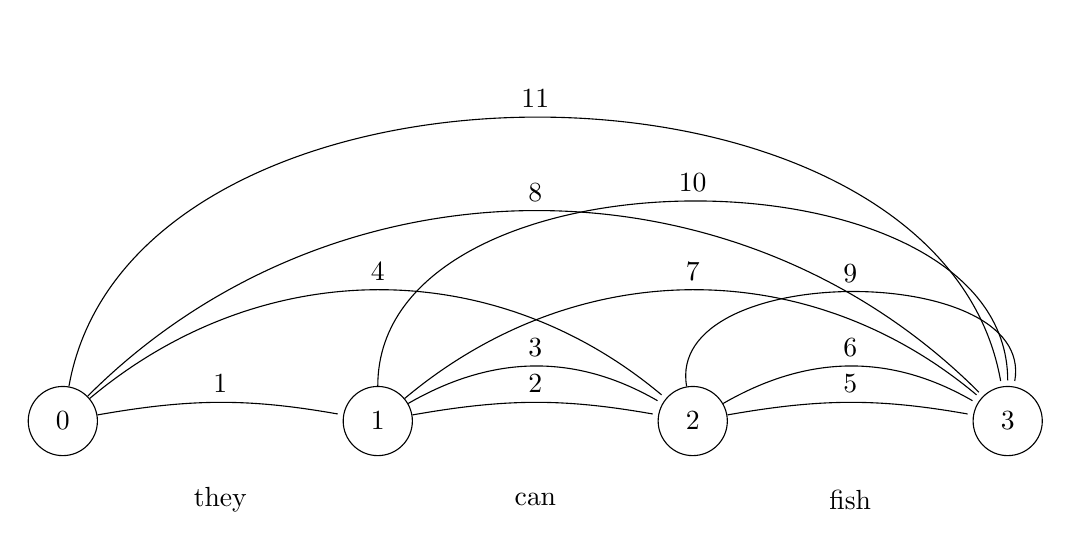
\begin{tikzpicture} [shorten >=2pt,auto,node distance=4cm]
      \node[state] (q1) {0};
      \node[state] (q2) [right of=q1] {1};
      \node[state] (q3) [right of=q2] {2};
      \node[state] (q4) [right of=q3] {3};
      
      \draw (2,-1) node (A) {they};
      \draw (6,-1) node  (B) {can};
      \draw (10,-1) node  (C) {fish};
      
      
      \draw (q1) to[bend left=10] node[auto] {1}(q2);
      \draw (q2) to[bend left=10] node[auto] {2}(q3);
      \draw (q2) to[bend left=30] node[auto] {3}(q3);
      \draw (q1) to[bend left=40] node[auto] {4}(q3);
      \draw (q3) to[bend left=10] node[auto] {5}(q4);
      \draw (q3) to[bend left=30] node[auto] {6}(q4);
      \draw (q2) to[bend left=40] node[auto] {7}(q4);
      \draw (q1) to[bend left=45] node[auto] {8}(q4);
      \draw (q3) to[bend left=100] node[auto] {9}(q4);
      \draw (q2) to[bend left=90] node[auto] {10}(q4);
      \draw (q1) to[bend left=80] node[auto] {11}(q4);
\end{tikzpicture}
\caption{Ermittelte Grammatikregeln durch Parsing zu "they can fish"}
\end{center}
\end{figure}

\subsection{Mängel kontextfreier Grammatiken}
Die Umsetzung der Modellierung von Sprache auf Basis kontextfreier Grammatiken ist mit einigen Problemem verbunden. Zunächst scheint es vorteilhaft, wenn durch die Rekursion alle möglichen Teildeutungen erfasst werden. Davon sind jedoch nicht alle sinnvoll und viele redundant. Es fällt auf, dass durch die Zerlegung in Teildeutungen durch Anwendung aller möglichen Regeln aus der Grammatik prinzipiell exponentiell viele Deutungen entstehen könnten. Teilweise würden auch grammatikalisch falsche Sätze akzeptiert, wenn nicht jeder Numerus, Kasus etc. eines Wortes als Terminalsymbol in der Menge an Produktionsregeln repräsentiert wird. In der obigen einfachen Grammatik wird \textit{"they fish"} genau so wie \textit{"it fish"} akzeptiert. 

Ferner werden Zusammenhänge aus Wörtern, die sich inhaltlich aufeinander beziehen, nicht abgebildet und nicht aus dem Kontext erfasst. Manche Verben erscheinen etwa ohne Berücksichtigung des Satzobjektes für den Menschen eher sinnlos. Der Teilsatz \textit{"Tom erwartet"} scheint unvollständig, die richtige Deutung von Zusammenhängen \textit{"Tom erwartet Max"} schließt den Kontext des Teilsatzes ein.

Eine Möglichkeit zur Lösung wird in Abschnitt 3.6 und 3.7 behandelt, indem die Kongruenz einer Formulierung ebenso wie Ansätze der Semantik bei der Deutung berücksichtigt werden. Dies ist mittels einfacher Produktionsregeln nicht möglich.

\section{Parsen mit constraint-basierten Grammatiken}
Wie zuvor an verschiedenen Beispielen demonstriert wurde, weisen die kontextfreien Grammatiken beim Parsen und Generieren einige Schwächen auf. Daher wird im folgenden Abschnitt ein neuer, komplexerer Ansatz vorgestellt, um sich mit den gleichen Problemen zu befassen. Kontextfreie Grammatiken können als constraint-basiert interpretiert werden, diese Bezeichnung ist jedoch üblicherweise mächtigeren Grammatiken vorbehalten. Constraint-basierte Grammatiken sind in NLP weit verbreitet und werden mit sogenannten feature-structures (Eigenschaftsstrukturen) dargestellt, daher auch oft feature-structure (FS) Grammatik genannt. Im folgenden Abschnitt soll die Umsetzung solch einer Grammatik durch FSs demonstriert werden.

FSs sind Graphen, welche große Ähnlichkeit zu Baumstrukturen aufweisen. Dabei haben sie  folgende Eingenschaften zu erfüllen:

\begin{enumerate}
\item Verbundenheit und einzelne Wurzel: jede FS hat genau eine Wurzel und alle anderen Knoten haben mindestens einen Elternknoten.
\item Einzigartigkeit der Eigenschaften: Knoten können einen beliebigen Ausgangsgrad haben, dabei muss jedoch jede Kante eine einzigartige Eigenschaft beschreiben sein.
\item Keine Kreise: kein Knoten darf direkt oder indirekt auf einen seiner Elternknoten zeigen. 
\item Werte: Nur Endknoten, also Knoten mit dem Ausgangsgrad 0, dürfen einen Wert enthalten. 
\item Endlichkeit: jede FS hat nur eine endliche Anzahl von Knoten.
\end{enumerate}

Ein Weg entlang von Eigenschaften wird als Pfad bezeichnet. Eigenschaften sind entweder atomar oder zusammengesetzt, abhängig davon, ob sie auf einen Endknoten, oder auf einen weiteren nicht-Endknoten zeigen.
Eine FS \textit{FS1} ist der FS \textit{FS2} untergeordnet, wenn \textit{FS2} mehr Informationen beinhaltet als \textit{FS1}. Dies wird durch die folgenden zwei Bedingungen sichergestellt:

\begin{enumerate}
\item Für jeden Pfad \textit{P} in \textit{FS1} gibt es einen gleichen Pfad \textit{P} in \textit{FS2}. Wenn \textit{P} in \textit{FS1} auf den Wert \textit{v} zeigt, so zeigt er auch in \textit{FS2} auf den Wert \textit{v}.
\item Jedes Paar von Pfaden \textit{P} und \textit{Q} mit Eintrittsinvarianz in \textit{FS1} habt auch Eintrittsinvarianz in \textit{FS2}.
\end{enumerate}

Die genaue Bedeutung der oben genannten Eigenschaften und Bedingungen soll anhand von Abbildungen und Beispielen genauer dargestellt werden. 

In dem folgenden, \cite{cop04} entnommenen Beispiel ist eine FS abgebildet, die sich in zwei Eigenschaften, \textit{"CAT"} für die Wortkategorie und \textit{"AGR"} für agreement (zu deutsch "Kongruenz"), teilt, welche jeweils auf die Endknoten mit den Werten \textit{"noun"} (für Nomen) und \textit{"sg"} (für Singular) zeigen. Die Eigenschaften \textit{"CAT"} und \textit{"AGR"} sind also atomar.

\begin{figure}[h!]
\begin{center}
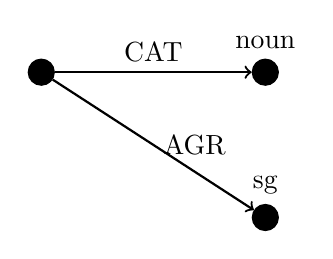
\begin{tikzpicture}
\node[draw,shape=circle,fill=black] (a) at (0,0) {};
\node[draw,shape=circle,fill=black,label=above:noun] [right = 2.5cm of a] (b) {};
\node[draw,shape=circle,fill=black,label=above:sg] [below = 1.5cm of b] (c) {};

\draw[thick, ->] (a) to node[midway, above] {CAT} (b);
\draw[thick, ->] (a) to node[midway, above, right] {AGR} (c);
\end{tikzpicture}
\caption{FS eines Nomens im Singular \cite{cop04}}
\end{center}
\end{figure}

Fügt man wie in der nächsten Abbildung vor der Wurzel eine weitere Eigenschaft \textit{"Head"} hinzu, so ist diese zusammengesetzt, da sie auf einen nicht-Endknoten zeigt. Dieser wird wiederum in die beiden Eigenschaften \textit{"CAT"} und \textit{"AGR"} aufgeteilt. 

\begin{figure}[h!]
\begin{center}
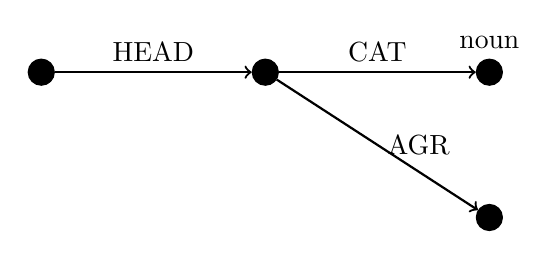
\begin{tikzpicture}

\node[draw,shape=circle,fill=black] (a) at (0,0) {};
\node[draw,shape=circle,fill=black,label=above:noun,right = 2.5cm of a] (b) {};
\node[draw,shape=circle,fill=black,below = 1.5cm of b] (c) {};
\node[draw,shape=circle,fill=black,left = 2.5cm of a] (d) {}; 

\draw[thick, ->] (a) to node[midway, above] {CAT} (b);
\draw[thick, ->] (a) to node[midway, above, right] {AGR} (c);
\draw[thick, ->] (d) to node[midway, above] {HEAD} (a);
\end{tikzpicture}
\caption{FS eines Nomens im Singular als HEAD zusammengefasst \cite{cop04}}
\end{center}
\end{figure}

Solche Strukturen lassen sich kompakter als attribute-value matrices (Attribut-Wert Matrizen, AVMs) aufschreiben. Die oben abgebildeten FSs sind wie folgt abzubilden:
\\
\begin{figure}[h!]
\begin{displaymath}
\begin{bmatrix} 
CAT & noun \\
AGR & sg 
\end{bmatrix} 
\end{displaymath}
\\
\begin{displaymath}
\bigg[
\begin{matrix}
HEAD &
\begin{bmatrix} 
CAT & noun \\
AGR & [] 
\end{bmatrix} 
\end{matrix}
\bigg]
\end{displaymath}
\caption{FSs aus Abb. 2.5 und 2.6 als AVM \cite{cop04}}
\end{figure}
\\

In FSs ist es möglich, dass mehrere Pfade den gleichen Endknoten erreichen, was als Eintrittsinvarianz bezeichnet wird. Sollte dies bei einem Endknoten zutreffen, so wird dessen Wert durch einen eingeklammerten Integer dargestellt. Der numerische Wert dieses Integers ist irrelevant, da er als Platzhalter für einen tatsächlichen grammatikalischen Wert verwendet wird. Dabei ist zu beachten, dass dann für gleiche Integer auch der gleiche Wert eingesetzt wird.

In der folgenden Abbildung sind Eintrittsinvarianz und FSs als AVMs dargestellt:
\\
\begin{table}[h]
\centering
\begin{tabularx}{320pt}{>{\centering\arraybackslash}m{3cm}|>{\centering\arraybackslash}m{3.7cm}|>{\centering\arraybackslash}m{3cm}}
%\begin{tabularx}{320pt}{>{\raggedright}c||c|c}
 & FS (als Graph) & AVM\\\hline\hline
Ohne Eintrittsinvarianz &   
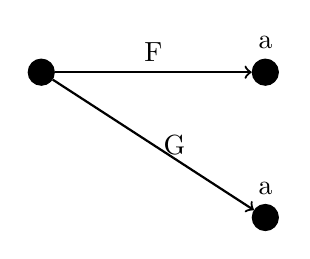
\begin{tikzpicture}
\node[draw,shape=circle,fill=black] (a) at (0,0) {};
\node[draw,shape=circle,fill=black,label=above:a] [right = 2.5cm of a] (b) {};
\node[draw,shape=circle,fill=black,label=above:a] [below = 1.5cm of b] (c) {};
\draw[thick, ->] (a) to node[midway, above] {F} (b);
\draw[thick, ->] (a) to node[midway, above, right] {G} (c);
\end{tikzpicture} & 
$\begin{bmatrix} 
F & a \\
G & a 
\end{bmatrix}$ 
\\\hline
mit Eintrittsinvarianz &
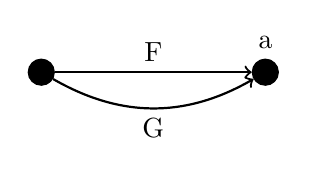
\begin{tikzpicture}
\node[draw,shape=circle,fill=black] (a) at (0,0) {};
\node[draw,shape=circle,fill=black,label=above:a] [right = 2.5cm of a] (b) {};
\draw[thick, ->] (a) to node[midway, above] {F} (b);
\draw[thick, ->] (a) [bend right] to node[midway, below] {G} (b);
\end{tikzpicture} & 
$\begin{bmatrix} 
F & [0] & a \\
G & [0]
\end{bmatrix}$ \\
\end{tabularx}\\
\caption{Eintrittsinvarianz als FSs und AVM \cite{cop04}}
\end{table}

Üblicherweise werden bei dem Umgang mit FSs viele zunächst simple FSs zu größeren vereint, um später aus einzelnen Wörtern korrekte, zusammenhängende Sätze oder Satzteile zu bilden. Diese Vereinigung (oder \textit{unification}) erlaubt es, alle Informationen der einzelnen FSs zu kombinieren. Leere eckige Klammern ([]) stehen dabei für einen bisher nicht spezifizierten Wert, welcher später gewählt und dann konsistent verwendet werden muss. Das genaue Vorgehen soll an dem folgenden Beispiel veranschaulicht werden:
\\

Die unten beschriebene constraint-basierte Grammatik fügt zusätzlich zu den Wortkategorien in der in 3.6.2 verwendeten Grammatik die Kongruenz zu den Produktionsregeln hinzu. Somit wird nicht nur auf die entsprechende Kategorie wie Verb oder Nomen, sondern auch auf die Multiplizitäten \textit{singular} und \textit{plural} geachtet. \newline
\\
\tt
1. S $\rightarrow$ NP-sg VP-sg\\
2. S $\rightarrow$ NP-pl VP-pl\\
3. VP-sg $\rightarrow$ V-sg NP-sg\\
4. VP-sg $\rightarrow$ V-sg NP-pl\\
5. VP-pl $\rightarrow$ V-pl NP-sg\\
6. VP-pl $\rightarrow$ V-pl NP-pl\\
\rm

Dementsprechend muss nun auch das verwendete Lexikon (als Produktionsregeln dargestellt) angepasst werden:\\
\\
\tt
NP-sg $\rightarrow$ he\\
NP-pl $\rightarrow$ fishermen\\
NP-sg $\rightarrow$ fish\\
NP-pl $\rightarrow$ fish\\
NP-pl $\rightarrow$ cats\\
VP-sg $\rightarrow$ catches\\
VP-pl $\rightarrow$ catch\\
VP-sg $\rightarrow$ fishes\\
VP-pl $\rightarrow$ fish\\
VP-sg $\rightarrow$ can\\
VP-pl $\rightarrow$ can\\
\rm

Mit den vorgestellten Änderung wird nun beispielsweise der Satz \textit{"He catch fish"} nicht mehr akzeptiert, da \textit{"He"}(singular) und \textit{"catch"}(in diesem Fall plural) über die ersten beiden Produktionsregeln an die gleichen Multiplizitäten gebunden sind. 
Dies lässt sich in der Darstellung der Grammatik durch AVMs besonders gut erkennen:\\

$\begin{bmatrix} 
CAT & S \\
AGR & [1]
\end{bmatrix} 
\rightarrow
\begin{bmatrix} 
CAT & NP \\
AGR & [1]
\end{bmatrix},
\begin{bmatrix} 
CAT & VP \\
AGR & [1] 
\end{bmatrix}$ \\

Diese AVM-Darstellung beinhaltet sowohl die erste, als auch die zweite Regel in der oben stehenden Grammatik, abhängig davon, ob der Platzhalter \textit{"[1]"} für den Wert \textit{"sg"} (singular) oder \textit{"pl"} (plural) steht. Das Einsetzen des Werts gilt nur innerhalb der Regel, die [1] kann also problemlos auch in anderen Regeln als Platzhalter verwendet und dort durch andere Werte ersetzt werden.\\

$\begin{bmatrix} 
CAT & VP \\
AGR & [1]
\end{bmatrix} 
\rightarrow
\begin{bmatrix} 
CAT & V \\
AGR & [1]
\end{bmatrix},
\begin{bmatrix} 
CAT & NP \\
AGR & [] 
\end{bmatrix}$ \\

Diese Regel enthält die gleichen Informationen wie die restlichen Produktionsregeln der obigen Grammatik, also 3., 4., 5. und 6., da für alle möglichen AGR-Werte von NP die nötige Produktionsregel existiert, solange die AGR-Werte von VP und V übereinstimmen. Die Regel ist also unabhängig von dem AGR-Wert bei NP, was es erlaubt, diesen Wert komplett unbelegt ("[]") zu lassen.

Die einzelnen Wörter bzw. Lexikoneinträge lassen sich durch simple AVMs wie folgt darstellen:\\

$\begin{bmatrix} 
CAT & NP \\
AGR & sg
\end{bmatrix}\rightarrow$ he \\

Man betrachte nun das Parsen des Beispielsatzes \textit{"He fishes"}. Die AVMs der Wörter \textit{He} und \textit{fishes} können über die erste Regel vereinigt werden. Für eine etwas präzisere Betrachtung nehme man an, dass Regeln aus Mutter (rechte Seite) und nummerierten Töchtern (linke Seite) bestehen. Somit sind die Tochter 1 \textit{He} und die Tochter 2 \textit{fishes} in der Mutter \textit{He fishes} wie folgt vereint:\\

$\begin{bmatrix} 
Mutter & \begin{bmatrix} 
CAT & S \\
AGR & [1] sg
\end{bmatrix} \\
Tochter 1 & \begin{bmatrix} 
CAT & NP \\
AGR & [1]
\end{bmatrix} \\
Tochter 2 & \begin{bmatrix} 
CAT & VP \\
AGR & [1]
\end{bmatrix}\\
\end{bmatrix}$\\

Da \textit{"He"} als singular erkannt wird, ist es nötig, dass auch alle anderen Kinder, in diesem Falle also nur "fishes", ebenfalls die [1] durch den Wert \textit{sg} ersetzen können. Falls dies möglich ist, kann die Vereinigung durchgeführt werden, was dann der [1] der Mutter ebenfalls den Wert \textit{sg} zuweist. Falls mehrere Vereinigungen durchzuführen sind, so macht die Reihenfolge keinen Unterschied, da immer das gleiche Resultat erzielt wird. Das Gleiche gilt für den verwendeten Pars-Algorithmus. Der einzige Unterschied ist, dass hier einige Algorithmen in bestimmten Fällen terminieren und andere nicht. 

Ohne eine entsprechende Produktionsregel wäre eine solche Vereinigung nicht möglich. Dies soll sowohl das Parsen, als auch Generieren von fehlerhaften Sätzen verhindern. In dem vorgestellten Beispiel reicht der Detailgrad der FSs jedoch nicht aus, um komplexere Sätze korrekt verarbeiten zu können.
Außerdem können mangelnde oder fehlerhafte Informationen in den verwendeten Lexika (und den daraus folgenden Produktionsregeln) für falsche Resultate sorgen. So ist etwa \textit{"fishes"} als singular gekennzeichnet, was es ermöglicht, den fehlerhaften Satz \textit{"I fishes"} zu parsen. Um dies zu verhindern wäre es nötig, nicht nur die Multiplizität, sondern auch die Person zu berücksichtigen. Je komplexer die in den FSs verwendeten Informationen, desto genauer und fehlerfreier lassen sich Sätze damit verarbeiten. Von einer vollständigen Grammatik ist man jedoch wie bereits erwähnt weit entfernt. 

\section{Lexikalische Semantiken und kontextbasierte Deutungen}
Mithilfe der im letzten Abschnitt eingeführten FSs wurde eine Möglichkeit vorgestellt, Abhängigkeiten zwischen einzelnen Wörtern abzubilden. Abgesehen von der Syntax, die durch eine möglichst gute Modellierung der zugrundeliegenden Grammatik im Computer darstellbar wird, ist es die Semantik, die den "Sinn" hinter einer Aussage repräsentiert. In NLP-Anwendungen wird dies häufig als "Logische Form" oder "Logik einer Aussage" umrissen (vgl. \cite{swb02}), wenn eine semantische Repräsentation eines Satzes erstellt werden soll. Einen Ansatz, um überhaupt solch einen Sinn abbilden zu können, bieten dabei die schon bekannten Feature Structures. Semantiken können theoretisch allesamt in einem Lexikon abgespeichert werden. Die korrekte Deutung kann dann anhand der bekannten Informationen aus der Semantik anderer Wörter bestimmt werden. Wenn man erneut das Problem von Verben mit und ohne erforderlichem Bezugswort betrachtet, damit diese Sinn ergeben, könnte diese Semantik als Erweiterung der FSs um die Argumente des Verbs erfolgen. Diese Repräsentation ist jedoch nur syntaktisch vollständig, sie erfasst beispielsweise keine der weiter unten genannten semantischen Feinheiten der Deutung. Es werden außerdem, logisch betrachtet, Quantoren benötigt, um das Ausmaß einer Aussage zu erfassen.

Zu starke Spezifizierungen der Semantik führen jedoch auch dazu, dass Mehrdeutigkeiten nicht mehr erfasst werden können. Wenn man die Relationen von Wörtern etwa durch die klassische Aussagenlogik abbildet, müssen diese auch unterschiedliche Semantiken liefern können.

\tt
Every man loves a woman.
\rm
\\
Zu deutsch \textit{"Jeder Mann liebt..."} ist semantisch mehrdeutig zwischen  
\begin{enumerate}
\item \textit{"...die eine Frau"}: $\exists y [woman'(y) \bigwedge \forall x [man'(x) \Rightarrow love'(x,y)]]$ und
\item \textit{"...irgendeine Frau"}: $\forall x [man'(x) \Rightarrow \exists y [woman'(y) \bigwedge love'(x,y)]]$
\end{enumerate}


Es stellt sich die Frage, ob hier also logisch betrachtet mehrere oder nur eine spezifische Frau gemeint ist. Die Regeln aus Symbolen der Aussagenlogik für die Semantik scheinen jedoch schon für den Menschen schwer erkennbar. In der Implementierung kann die Deutung eingeschränkt werden, wie im nächsten Abschnitt beleuchtet wird.

\subsection{Meaning-Postulates und Vereinfachung}
Gesamtzusammenhänge werden immer dann offensichtlich, wenn aus einem Teil mehr als nur das übersetzte Wort abgeleitet werden kann. Die Bedeutung wird immer dann klarer, wenn sich eine Aussage über den Zusammenhang treffen lässt. Umgangssprachlich nutzt man beim Herstellen solcher Zusammenhänge bestimmte Metainformationen, also Wissen, dass über die reine Wortbedeutung hinausgeht. Die Schlussfolgerung einer Bedeutung wird somit vereinfacht, da die Möglichkeiten eingeschränkt sind. Für die Abbildung von Semantik auf logische Formeln stellen die in Abschnitt 3.1.5 beschriebenen $\in_T$-Logiken einen Ansatz dar, dies zu formalisieren. Im folgenden werden daher zur Erläuterung Teile dieser Notation benutzt. Der Philosoph Rudolf Carnap hat schon 1952  untersucht, wie man den Sinn hinter dem geschriebenen Wort durch Vereinfachung erfassen kann. 
\begin{enumerate}
\item \textit{Meaning-Postulates}: A beinhaltet B und C

Mithilfe von \textit{Meaning-Postulates} können Thesen zur Deutung vorgenommen werden, etwa das Beispiel aus \cite{car52}:

$\forall x[bachelor(x)\Rightarrow man(x)\bigwedge unmarried(x)]$
sinngemäß: Ein Junggeselle ist ein Mann und nicht verheiratet.

Es ist zu beachten, dass diese Thesen nicht allzu vereinfachend ausfallen und deren Korrektheit ist darüber hinaus nicht in jeder Situation gewährleistet. Naiv könnte man davon ausgehen, dass die obige These auch mit Äquivalenz statt nur Implikation eine korrekte Semantik bildet. \cite{car52} beobachtet etwa, dass die Eigenschaften rechts davon zwar auch für den Papst gelten, jedoch scheint die Deutung als Junggeselle recht unpassend.

\item \textit{Hyponomy}: A ist ein B

Bei der Frage nach Zusammenhängen kommt unwillkürlich die Frage auf, welche Eigenschaften hinter der Bedeutung eines Worts stehen. 

\tt
Ein Hund ist ein Tier. 
\rm
also hat ein Hund auch alle Eigenschaften eines Tieres.

Durch Kategorisierung können verschiedene Ausprägungen  der gleichen Sache zusammengefasst werden; Die Erfassung von Hyponomien ist nach \cite{cop04} wesentlich für Semantiken in NLP.

\item \textit{Meronymy}: A $\subseteq$ B, A ist Teil von B

\item \textit{Synonymy}: A $\equiv$ B, A ist semantisch äquivalent zu B

\item \textit{Antonymy}: A $\equiv \neg$B, A bedeutet das Gegenteil von B

\end{enumerate}

Diese Vereinfachungen sind Ansätze zur verbesserten Erfassung der Semantik. WORDNET Jedoch stellt sich für die Praxis etwa die Frage, ob diese auch für Verben und Adjektive oder Nomen wie \textit{"Gedanke"}, die sich schlecht verbildlichen lassen, getroffen werden können, ob es "Mehrfachvererbung" (Hund als Haustier und als Vierbeiner) gibt, oder wo der Ursprung aller Kategorien liegt. Wenn Wörter einer Kategorie zugeordnet werden, können feine Nuancen zwischen verschiedenen Wörtern verloren gehen.

\subsection{Umgang mit Semantik in der Anwendung}
Besonders in Arbeiten wie QUELLEN aus den 1980er Jahren versuchte man, Semantiken besser als durch einfache FSs zu erfassen, um etwa eine korrekte Negation in der Semantik abzubilden. Es ist dazu jedoch nicht nur erforderlich, alle möglichen Semantiken vorher in einem Lexikon parat zu haben, sondern auch, auf Basis der Textinformation eine davon als die wahrscheinlich richtige zu identifizieren. Die allgemeine Lösung dieses Problems ist AI-Vollständig. 

In der Implementierung bedarf es daher Möglichkeiten, überabzählbare Mehrdeutigkeiten und vage Formulierungen zu verhindern. Mögliche Semantiken müssen dahingehend beschränkt werden, dass das Problem dann nicht mehr AI-Vollständig ist, da immer eine eindeutige Lösung gefunden wird. Es wird also beispielsweise erfasst, in welchen Wortkombinationen ein mehrdeutiges Wort häufig auftritt, um eine Beziehung daraus abzuleiten. 

Übersetzungsprogramme nutzen dies etwa aus, um eine sinnvolle Deutung des Eingabetextes für die Übersetzung zu erreichen. Taucht in einem Text etwa das Wort \textit{Bank} in Verbindung mit anderen Wörtern aus dem Finanzwesen auf, ist klar, dass ein \textit{Geldinstitut} gemeint ist. Die Deutung als \textit{Bank} als \textit{Sitzgelegenheit} wäre in Verbindung mit diesem Text dann unpassend, aber im Zusammenhang mit \textit{sitzen} naheliegend. 

Nach \cite{car52} existieren bei der Zuordnung einer Semantik eines Satzes in der Welt weitere Probleme, die durch mehrdeutige Semantik verursacht werden. Eines dieser Probleme ist \textit{Polysemy}. 

Das bekannte Beispiel von \textit{Bank} (als Geldinstitut) vs. \textit{Bank} (als Parkbank) kann in der Regel durch die Herleitung der Semantik durch andere Wörter aufgelöst werden, da die Menge der Bedeutungen komplett disjunkt sind. Umso schwieriger wird es, wenn etwa eine dritte Bedeutung \textit{Bank} (als Spielbank im Casino) hinzukommt, deren Bedeutung sich inhaltlich mit der des Geldinstituts überschneidet. 

Ein weiteres Beispiel ist etwa \textit{"Max mag Kartoffeln"}, das eine rohe Kartoffel, Salzkartoffeln, Kartoffelpflanzen und mehr meinen kann. Die Spezifizierungen weisen zwar auch Gemeinsamkeiten auf, haben jedoch eine andere Bedeutung. Die Formulierung Kartoffel ist also vage.
Man beschränkt sich daher oft nur auf eine flache Semantik, also nur auf einfache Zusammenhänge. In der Praxis begrenzt man die Semantik jedoch auch auf eine überschaubare Wissensbasis, genannt \textit{"Ontologie"}, sodass der Kontext strikt vorgegeben und somit eindeutiger ist.

\begin{figure}
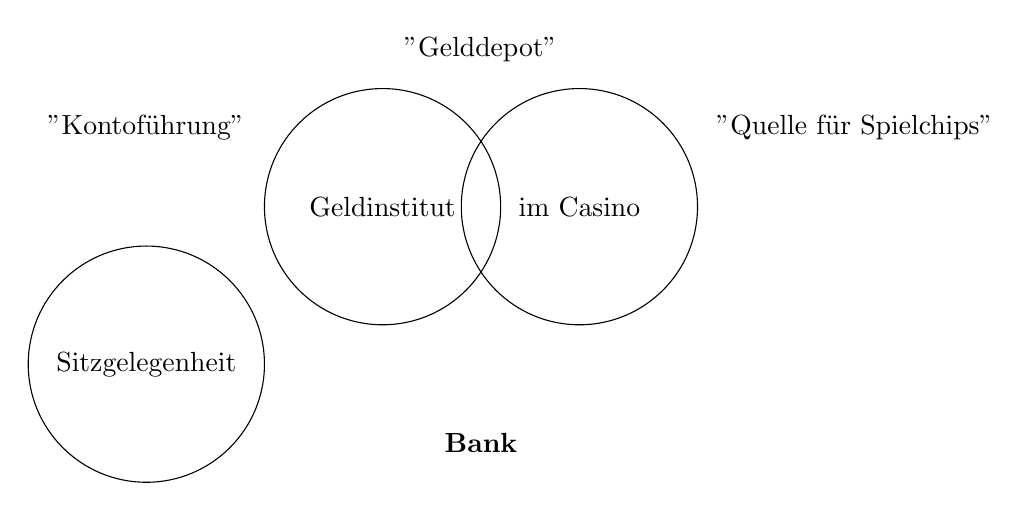
\begin{tikzpicture}
\draw (3,0) circle (1.5cm) node {Geldinstitut};
\draw (5.5,0) circle (1.5cm) node {im Casino};
\draw (0,-2) circle (1.5cm) node {Sitzgelegenheit};
\node at (0,1) {"Kontoführung"};
\node at (4.25,-3) {\textbf{Bank}};
\node at (4.25,2) {"Gelddepot"};
\node at (9,1) {"Quelle für Spielchips"};
\end{tikzpicture}
\caption{mögliche Bedeutungsmengen eines Polysems}
\end{figure}

\subsection{Auflösung von Mehrdeutigkeiten durch Semantiken}
Wie bereits beschrieben, stellen Mehrdeutigkeiten bei unbegrenzter Anwendungsdomöne ein ernstzunehmendes Problem dar, da schlicht zu viele mögliche Deutungen existieren. In der Praxis sammelt man daher Fachwissen aus der Problemdomäne und speichert es in Form von Ontologien zu Wissensbasen ab. Der Prozess der Auflösung von Mehrdeutigkeiten wird als Word-Sense-Disambiguation (kurz WSD) bezeichnet. Frühe WSD-Systeme basierten noch auf von Hand eingetragenen Deutungen (vgl. POS-Tagging). Heutige Systeme auf Basis von Machine-Learning können jedoch auf Basis eines kleinen Semantik-Corpus entweder selbstständig neue Bedeutungen erlernen oder verfügen über ein gesondertes Lexikon von ausführlichen Informationen zur Auflösung von Mehrdeutigkeiten. 

Wortkombinationen, in denen mehrdeutige Wörter auftauchen, werden als \textit{Collocation} bezeichnet. Die syntaktische Analyse identifiziert alle Wörter, die auf das mehrdeutige Wort bezogen sind. Mithilfe der syntaktischen Analyse können dann die klaren Bedeutungen zugeordnet werden, wie das Beispiel aus \cite{cop04} zeigt:

\tt
Striped bass are common.

Bass guitars are common.
\rm

Die Mehrdeutigkeit liegt darin, dass es sich nach dem Lesen des ersten Satzes um gestreifte Barsche, oder um gestreifte Bass(-gitarren) handeln kann. Collocation untersucht nun, ob bass noch in anderen Phrasen auftaucht (bass guitars ist eindeutig).

Für die Erstellung eines Lexikons, mit dessen Hilfe mehrere Bedeutungen zugeordnet werden können, ist Collocation hilfreich. Machine Translation kann damit automatisiert Mehrdeutigkeiten erlernen, jedoch ist die Fehlerquote ohne Einschränkung recht groß und Wörter können auch uneindeutig erscheinen. Yarowsky beschreibt in \cite{yar95} solch ein Verfahren zur Sammlung von Mehrdeutigkeiten, genannt \textit{Unsupervised Learning}, wie folgt: 

\begin{enumerate}
\item Zunächst werden alle Sätze, indem das mehrdeutige Wort auftaucht, aus dem Text aufgelistet.
\item Collocations aus dem Wort mit völlig unterschiedlicher Bedeutung des Bezugswortes werden als aufgelöst gekennzeichnet. Die möglichen Deutungen werden in das Lexikon eingetragen. Diese meinen eindeutig immer etwas Anderes, da der Sachzusammenhang anders ist.
\item Eine decision list wird erstellt, die die noch nicht aufgelösten Stellen, an denen das Wort auftaucht, zu den in 2. ermittelten Bedeutungen einordnet. Dabei wird die Wahrscheinlichkeit der Zugehörigkeit ermittelt. Dies kann etwa der nächste Abstand zu einer eindeutig identifizierten Semantik sein.
\item Die Einträge aus der decision list mit der höchsten Wahrscheinlichkeit werden auf jeden EIntrag angewendet. Dabei wird unterhalb einer Toleranzgrenze festgelegt, die festlegt, ab welcher Abweichung von der Wahrscheinlichkeit die Zuordnung noch nicht eindeutig ist. 
\item Ab Schritt drei wird solange wiederholt, bis alle Wörter einer Bedeutung zugeordnet wurden.
\end{enumerate} 

Ähnlich wie die eingangs vorgestellten Corpora zur Sammlung von Syntax, stellt solch ein Lexikon dann eine Ontologie dar, also eine Sammlung von Wissen. Implentierungsbeispiele aus \cite{col11} erläutern, wie die Zuordnung von Bedeutungen zu Wörtern (Semantic Role Labelling) und die Darstellung von Wissensverknüpfungen in Vektoren erfolgt. Allgemeines Wissen über die Welt sollte dabei ebenso Teil der Wissensbasis sein, wie fachspezifisches Wissen aus der Anwendungsdomäne. Dieses tiefere Wissen kann dann zur Auflösung von Mehrdeutigkeiten herangezogen werden.

\section{Kontext}
In vielen Fällen ist für ein semantisches Verständnis von natürlicher Sprache der Kontext ausschlaggebend. Der folgende Abschnitt beschäftigt sich mit kontextabhängigen Informationen, deren Auswirkung und Extraktion. 

\subsection{Bezugsausdrücke}
Viele Worte haben selbst keinen klaren semantischen Inhalt, nehmen jedoch Bezug auf andere Worte, über welche sie ihre Bedeutung erhalten. Dazu gehören beispielsweise Pronomen. Der Ausdruck \textit{"Er"} hat keinerlei Ausdrucksstärke, wenn er sich nicht auf eine tatsächliche Instanz wie \textit{"Max Mustermann"} beziehen kann.

\tt
Das ist Max Mustermann. Er ist glücklich.
\rm

Hier erhält das Pronomen \textit{"Er"} dieselben semantischen Informationen wie \textit{Max Mustermann} und ließe sich ersetzen, ohne dass semantische Informationen verloren gehen. Man weiß also sofort, dass Max Mustermann glücklich ist. Für eine besseres Verständnis der Funktionsweise von Bezugsausdrücken sind zunächst die folgenden Begriffe zu klären:

\begin{enumerate}
\item Referent/Bezug: Eine tatsächliche Instanz (in der echten Welt) auf die sich andere Satzteile beziehen (hier eine bestimmte Person)
\item Beziehender Ausdruck: Ausdruck, der sich auf einen Referent bezieht (hier "Er")
\item Bezugswort: Teil des Textes auf den sich ein beziehender Ausdruck bezieht (hier Max Mustermann)
\item Anaphora: Der Bezug auf einen Antezedent (hier würde man "Er" als anaphorisch bezeichnen, da es sich auf den Antezedent Max Mustermann bezieht.) 
\end{enumerate}

Üblicherweise wird in einem Text zunächst ein Referent über eine Bezugswort eingeführt und später über beziehende Ausdrücke referenziert. Es ist jedoch auch möglich, erst einen beziehenden Ausdruck zu verwenden und den Referent erst später zu erwähnen:

\tt
Weil er so glücklich war, musste Max lachen.
\rm

Es ist für Pronomen möglich auf keinerlei Referent zu verweisen. Diese Pronomen werden als pleonastisch bezeichnet und üblicherweise verwendet und einen generellen Zustand zu beschreiben:

\tt 
Es ist schönes Wetter, weil es nicht regnet.
\rm

\subsection{Kohärenz}
Sätze müssen eine inhaltliche Verbindung haben um kohärent zu sein. Einzelne Sätze können abgeschlossen sein, jedoch irritieren, wenn sie hintereinander stehen. 

\tt 
Das ist Max Mustermann. Tom ist glücklich.
\rm

Fügt man einen Satz mit verbindender Funktion hinzu, so mag es zwar ungewöhnlich formuliert, doch definitiv sinnvoller sein. (Es würde für den Leser der Sätze reichen, wenn er den Kontext bereits kennt, ohne das dieser mit übermittelt wird. Dies ist jedoch nur im Zusammenhang mit Ontologien interessant.)

\tt 
Das ist Max Mustermann. Er hat Tom ein Fahrrad geschenkt. Tom ist glücklich.
\rm

Kohärenz kann maßgeblich Einfluss auf die Bedeutung eines Satzes nehmen:

\tt Max ist ein Freund von Tom. Er hat ihm ein Fahrrad geschenkt. 

\rm

Zwei verschiedenen valide Interpretationen sind:

\begin{enumerate}
\item Max hat Tom ein Fahrrad geschenkt, weil sie Freunde sind.
\item Max ist ein Freund von Tom, weil Tom ihm ein Fahrrad geschenkt hat. 
\end{enumerate}

\subsection{Präferenz von Referenten}
In vielen Fällen kann ein beziehender Ausdruck auf verschiedene zuvor eingeführte Referenten verweisen. Hierbei sind die folgenden Regeln zu beachten:

\begin{enumerate}
\item Nähe: Das nähere Bezugswort ist üblicherweise der Referent. \textit{"Er"} bezieht sich also auf \textit{Tom}.\\
\tt Max hat ein Fahrrad. Tom hat auch ein Fahrrad. Er leiht es manchmal Tim.
\rm
\item Grammatikalische Rolle: Man geht von einem Bezug auf Subjekte, dann Objekte und dann erst andere Satzteile aus. \textit{"Er"} bezieht sich also auf \textit{Max}.\\
\tt
Max fährt mit Tom Fahrrad. Er ist sehr schnell.
\rm
\item Wiederholtes Erwähnen: Ein wiederholtes Bezugswort ist höchstwahrscheinlich der Referent. \textit{"Er"} bezieht sich also üblicherweise auf \textit{Tom}.\\
\tt
Tom fährt Fahrrad. Max fährt mit Tom. Er ist sehr schnell.
\rm
\item Parallelismus: Bezugswörter mit gleicher oder ähnlicher Funktion wie der beziehende Ausdruck werden bevorzugt. \textit{"ihn"} bezieht sich also auf \textit{Tom}. \\
\tt
Max fährt mit Tom Fahrrad. Morgen fährt Tim mit ihm Auto.
\rm
\item Kohärenzeffekte: Der Inhalt des Kontextes kann entgegen der obigen Regeln den Bezug auf einen bestimmten Referent nahelegen. \textit{"Er"} bezieht sich also auf \textit{Tom}, da Hilfsbereitschaft als Erklärung dienen kann, warum andere ihn mögen.\\
\tt
Tom wird sehr von Max gemocht. Er ist immer nett und hilfsbereit.
\rm
\end{enumerate}
Ein verwendeter Algorithmus zur Auflösung von Pronomen-Präferenzen wird in \cite{ll94} von Lappin und Leass vorgestellt.\\

\chapter{Anforderungsanaylse von NLP-Problemen}
Das folgende Kapitel beschäftigt sich mit der Anfolderungsanalyse NLP-Tools genrell. Dabei gibt es eine Vielzahl von Anforderungen und Anforderungsbereichen die zu berücksichtigen sind. Zunächst sind natürlich alle generellen Anforderungen zu Verarbeitungsprogrammen relevant. Des weiteren erwachsen jedoch aus den Eigenschaften von NLP bestimmte Probleme, welche wiederum speziellere Anforderungen notwendig machen. Dieses Kapitel wird sich nicht auf ein bestimtes Tool beziehen, sondern durch die Darstellung der besagten Anforderungen eine Grundlage für das nächste Kapitel liefern, in welchem GATE anhand der hier aufgeführten Punkte evaluiert wird. 

Zunächst werden die oben erwähnten Eigenschaften von NLP betrachtet und die resultierenden Probleme aufgezählt. Daraufhin werden die genrellen und spezifischen Anforderungen an NLP-Tools ausgeführt. Diese sind in funktionale und nicht-funktionale Anfoderungen unterteilt, welche wiederum in bestimmte Anforderungsbereiche wie zum Beispiel "Design" oder "Sicherheit" aufgeteilt sind.

\section{Eigenschaften von NLP}
In diesem Abschnitt werden die in dem vorherigen Kapitel dargestellten Eigenschaften von NLP noch einmal kurz aufgeführt. Der Fokus liegt dabei auf den Eigenschaften, welche bei der Anforderungsanalyse besonderen Einfluss haben. Eine Auflistung der für uns relevantesten Eigenschaften kann wie folgt aussehen:

\begin{enumerate}
\item Ständiger Wandel von Sprache: natürliche Sprache verändert sich konstant. Dies gilt sowhl für Morphologie, als auch für Syntax, was wiederum zu variierenden Semantiken zwei gleicher Sätze zu einem unterschiedlichen Zeitpunkt führen kann. Dies hat zur Folge, dass Fehler entstehen, wenn NLP-Tools nicht ausreichend wartbar sind oder nicht immer Zugriff auf den aktuellsten Stand der Sprache haben, z.B. über Lexika.
\item Vielzahl von Verarbeitungsschritten: Für eine ausreichende linguistische Analyse von Texten werden viele Arbeitsschritte hintereinander druchgeführt, wie in Abschnitt 2.2.1 beschrieben wird. Im Gegensatz zu vielen Programmierumgebungen reicht es also nicht einfach ein Programm zu kompilieren. Eingie Verarbeitungsschritte werden zudem noch den eigenen Zwecken angepasst um bestimmte Ergebnisse zu erziehlen. Dies muss also durch ein NLP-Tool ermöglicht und so gut es geht vereinfacht werden.
\item Hohe Laufzeiten: Bei der Verarbeitung von Texten kann es zu sehr hohen Laufzeiten kommen. Diese sind bspw. abhängig von der Länge des Textes, der Anzahl der Verarbeitungsschritte und den in diesen verwendeten Algorithmen. Ein NLP-Tool sollte also über entsprechende Funktionalitäten verfügen, um die Laufzeit überblicken und evtl. einschränken zu können. 
\item Domäne und Präzision: Bei NLP ist in vielen Fällen abzuwägen zwischen einer präzisen und schnellen Verarbeitung in kleiner Domäne (kleine Lexika, Corpora, semantisches Umfeld usw.) oder einer langsameren, weniger präzisen Verarbeitung in einer dafür größeren bzw. generelleren Domäne. Ein NLP-Tool muss es also ermöglichen die verarbeitungsdomäne jedes mal selbst zu wählen.
\end{enumerate}

Die hier nur kurz angerissenen Anforderungen, welche aus diesen Eigenschaft entstehen, werden im folgenden Abschnitt jeweils einzeln genauer behandelt.

\section{Anforderungen für die Entwicklung von NLP-Tools}
Wie bereits im vorigen Abschnitt dargelegt wurde, sind bei der Entwicklung von Tools, die NLP-Algorithmen zur Auswertung von Sprache verwenden, Besonderheiten zu beachten. Daraus ergibt sich besonders im Hinblick auf die korrekte Umsetzung der Funktionalität der Software Handlungsbedarf für die Planung der Entwicklung und das Anforderungsmanagement. Diese Anforderungen lassen sich im Sinne der Softwaretechnik in der Planung der Entwicklung in funktionale und nicht-funktionale Anforderungen an eine Software gliedern. Im Bereich der Softwareentwicklung existieren mittlerweile standardisierte Typen von Anforderungen, die in der DIN 9126 zusammengefasst sind. In QUELLE sind diese zu finden, jedoch fällt die Umsetzung besonders in Anwendungsgebieten, die in denen immer wieder neue Ansätze entstehen, nicht leicht. Da Komponenten für NLP ständig mit neuen Algorithmen implementiert werden können, fehlen mitunter best-practices für deren Entwicklung.

In diesem Abschnitt soll besonderer Fokus auf der Benennung und Einordnung besonders beachtenswerter Anforderungen, die sich bei NLP ergeben, auf der DIN-Norm 9126 gelegt werden. In der Spezifizierung einzelner Anforderungen werden dabei die inhaltlichen Grundlagen aus Kap. 2 genutzt, um die Problematiken zu motivieren und darzulegen. Mögliche Schwachpunkte im Entwicklungsprozess können somit bereits im Vorhinein identifiziert und vermieden werden. Es ist dabei zu beachten, dass durch die hohe Abhängigkeit von NLP zum Anwendungskontext in verschiedenen Domänen noch weitere Anforderungen entstehen können. Wenn etwa die Semantik besonders im Vordergrund steht oder schwer fachspezifisches Wissen erforderlich ist, muss man schon beim Programmentwurf auf diese Besonderheiten eingehen.

\subsection{Funktionale Anforderungen}
Im Kontext der Entwicklung von NLP-Tools können konkrete Anforderungen an den Betriebsablauf erhoben werden. Funktionale Anforderungen beschreiben, was das Endprodukt, also hier die hergestellte Software, zweckmäßig tun soll. Obwohl diese Anforderungen in der Regel spezifisch für einen Entwicklungszyklus festgelegt werden, existieren bei NLP auch allgemein besondere funktionale Anforderungen. Die hier skizzierte Liste von Anforderungen dient dabei zunächst zur Orientierung vor der Implementierungsphase, erhebt jedoch keinen Anspruch auf Vollständigkeit und ist für die Entwicklung erweiterbar. Je nach Entwicklungsparadigma und Anwendungskontext können sich die Anforderungen ändern. Aufgrund der in Kap. 2.2 vorgestellten Schritte der Linguistischen Analyse existieren allgemein u.a. folgende Anforderungen an den Funktionsumfang:
\begin{enumerate}
\item Die Software muss standardisierte Dateitypen einlesen können.

In der Softwareentwicklung ist eine hohe Flexibilität der späteren Einsatzmöglichkeiten von Software anzuraten. Wenn eine möglichst universell einsetzbare Software eingesetzt werden soll, muss sie daher in der Anwendungsdomäne häufig benutzte Dateiformate akzeptieren. Dies umfasst ganz konkret etwa .txt oder .doc Dateien als häufig vorkommende Dateitypen für Texte, kann aber individuell erweiterbar sein. Beim Einsatz in einer leicht anderen Umgebung kann durch Erweiterung der Textverarbeitung aber beispielsweise auch Speech-to-Text, realisiert werden. Dazu muss dann auch ein Parser für Audiodateien wie .wav oder .mp3  in einen Text integriert werden.

\item Die Verarbeitungslogik der Programme muss in Modulen (getrennten Diensten) mit standardisierter Datenübergabe erfolgen (siehe Abschnitt 3.1.2.): 

Wie bereits zu Beginn von Kap. 2 dargelegt wurde, sind bei der Verarbeitung von Sprache verschiedene Teilschritte in der Verarbeitung erforderlich, die jeweils unterschiedliche Logiken und Aspekte von Sprache umsetzen und verarbeiten. Diese Schritte sind im fertigen Programm dann als Algorithmen implementiert, die teils vollkommen unterschiedlich arbeiten. Daher muss schon die Implementierung in eigenständigen Modulen erfolgen, sodass diese später auch einfach ausgetauscht werden können.

Die Weitergabe der Verarbeitungsergebnisse der Module an das jeweils nächste muss ebenfalls standardisiert erfolgen, damit die Schritte durch Anwender nachvollzogen werden können. Informationen und Taggings von Textstellen können etwa über XML oder einen eigens entwickelten Dokumententyp ausgetauscht werden. Damit sind sie dann für jedes Modul in der Verarbeitungskette les- und erweiterbar, wenn neue Informationen aus dem Text gewonnen werden.

\item Der Nutzer muss Programmmodule für die Verarbeitung konfigurieren können, sodass das Programm individuell arbeitet.

Je nach gewünschter Funktionalität müssen die einzelnen Module durch den Nutzer weiter konfigurierbar sein, sodass das gewünschte Ergebnis erreicht wird. Bei der Generierung von Taggings benötigt man etwa eine Funktion zum filtern, wenn nach Wörtern mit dem entsprechenden Tagging gesucht werden soll. Auch muss es möglich sein, sich jeden Teilschritt einzeln in einer entsprechenden log-Datei ausgeben zu lassen, um eventuelle Fehler in der Verarbeitung rechtzeitig zu erkennen. Dies könnte etwa wieder eine .txt Datei sein, die entsprechend formatierten Text enthält.

Beim Einsatz von Algorithmen in Modulen ist es teilweise erforderlich, dass domänenspezifische Trainingsdaten verwendet werden (siehe bspw. Abschnitt 2.4). Je nach Anwendungskontext des NLP-Tools enthalten diese Trainingsdaten dann andere Stammdaten bzw. Corpora, damit die Module besser für spezifische Texte eingesetzt werden können. Dazu ist es erforderlich, dass der Nutzer diese Datensätze selbst wählen und in das Programm laden kann.

\item Die Software muss die Sprachauswertung im Ergebnis so darstellen können, dass wesentliche Textstellen und Annotationen markiert sind. 

Durch die sogenannte \textit{Annotation} von Text liegt im Ergebnis der Software ein gekennzeichneter Text vor, der Anmerkungen zur Deutung des Textes enthält. Die Einordnung von Wörtern und Sätzen anhand von Grammatikregeln muss klar ersichtlich sein. Für den Anwender ist es relevant, dass es dabei standardisierte Darstellungen von Deutungen im Programm gibt; jede Annotation eines Typs muss einheitlich und besonders hervorgehoben sein. Die Ergebnisdarstellung kann dabei graphisch für den Benutzer erfolgen, indem entsprechende Textstellen beispielsweise farbig markiert werden. Dies ist jedoch nicht notwendigerweise erforderlich, wenn das NLP-Tool etwa nur einen Teil der Verarbeitungskette ausmacht oder dessen Output nicht manuell verifiziert werden soll. Im Ergebnis könnte also auch etwa eine XML-Datei, die Taggings zu Textstellen mit der Kategorie der Annotation enthält, vorliegen.

\item Programmverhalten bei sprachlichen Uneindeutigkeiten wird berücksichtigt und definiert.

Die Basis für eine Vielzahl von Problemen beim Entwurf von Verarbeitungslogik für NLP-Tools stellen sprachliche Mehrdeutigkeiten dar. Die Bewältigung solcher Mehrdeutigkeiten ist daher ein wesentlicher Bestandteil der Programmmodule und ein Auswahlkriterium, ob eine Implementierungsmöglichkeit geeignet ist. Das Programmverhalten bei solchen Mehrdeutigkeiten erzeugt mitunter mehrere plausible Ergebnisse bzw. Pfade. Da Programme, die NLP nutzen, aber deterministisch sein müssen (siehe nicht-funktionale Anforderungen), muss es an solchen Zweigstellen keinesfalls abbrechen und evtl. auf Basis von Heuristiken eine Möglichkeit für die weitere Verarbeitung auswählen. Alternativ könnte das Programm auch durch Interaktion mit dem Anwender zunächst meherere Möglichkeiten anbieten und diese in einem Dialogfenster anzeigen. Der Benutzer kann dann eine davon Auswählen, mit der das Programm die Verarbeitung fortsetzt. Wenn etwa das Beispiel aus Kap.2 \textit{they can fish} vorliegt.
Durch 

\item Die Software muss jederzeit manuell terminierbar sein (siehe Abschnitt 3.1.3.).

Aufgrund der Vielzahl von Verarbeitungsschritten von NLP kann davon ausgegangen werden, dass bei der Analyse langer und komplexer Dokumente eine hohe Programmlaufzeit erreicht wird. Daher muss jederzeit auch die Terminierung durch den Benutzer möglich sein, wenn dies durch Umstände im Einsatzumfeld erforderlich ist. Es ist realistisch, dass etwa mehrere Implementierungen parallel genutzt werden und nicht alle Ergebnisse benötigt werden. 
Daher muss es für den Nutzer etwa einen Button geben, der den unkomplizierten Programmabbruch ermöglicht. Dabei dürfen jedoch keinesfalls sensible Daten verloren gehen bzw. beschädigt werden. 
Es muss dabei also besonders darauf geachtet werden, dass die Programmoperationen atomar sind und sich Teilschritte mit einer Zurück-Funktion rückgängig machen lassen, ohne dass die Quelldaten beschädigt werden. Ein (Teil-)Rollback wird somit vereinfacht.

\item Die Software ermöglicht das Einbinden von Plug-Ins

Durch die im vorigen Abschnitt beschriebene Weiterentwicklung von Sprache, aber auch durch den Entwurf neuer Algorithmen und den Wunsch nach neuen Funktionen der Software muss es eine standardisierte Schnittstelle zur Einbindung von Plug-Ins geben. Die Basisfunktion der Software ist dann die Annotation, ergänzend kommen dann weitere Funktionen hinzu, die diese nutzen. Die Plug-Ins können dann in den Funktionsablauf und Modulhierarchie der Software integriert werden. So können durch die unter Punkt 2 beschriebene Standardisierung der Ausgabe einfach neu entstandene Module in der Kette eingefügt werden, ohne dass andere Module davor oder danach angepasst werden müssen.

\item Die Software stellt Möglichkeiten zur Erstellung eigener Plug-Ins

Um betriebsabhängig weitere Funktionen im Programm umzusetzen, muss das NLP-Tool Möglichkeiten zur Eigenentwicklung bieten. Dies kann entweder mittels einer eigenen Entwicklungsumgebung (IDE) umgesetzt werden, oder mit einer Schablone für andere Programmierumgebungen für Sprachen wie beispielsweise JAVA. Aus dem NLP-Programm hinaus lässt sich ein Funktionseditor zur Erstellung dieser Plug-Ins aufrufen. Das Tool sollte die Entwicklung in einer Programmiersprache, die den Endanwendern bereits bekannt ist, anbieten. Somit könnten etwa neue Funktionalitäten beispielsweise in JAVA implementiert werden, die dann durch die Umsetzung von Punkt 6 standardisiert geladen werden.

\item Die Software kann automatisiert in einen größeren Workflow eingebunden werden

Vor und nach dem Einsatz von NLP-Software müssen die Daten über eine standardisierte Schnittstelle zur Verfügung stehen. Im betrieblichen Kontext kommen meist mehrere Programme in einem Arbeitsbereich zum Einsatz. Nach der Linguistischen Analyse durch ein NLP-Tool kann etwa die weitere Verarbeitung der Ergebnisse im Anwendungskontext erfolgen, also die Weiterverarbeitung der Daten aus dem NLP in anderen Programmen. Ergebnisse müssen weiter aufbereitet werden können, etwa zur Visualisierung oder Speicherung. Die Software muss also in der Lage sein, Datenein- und -ausgabeströme bereit zu stellen und auch zu verarbeiten. 
\end{enumerate}

\subsection{Nicht-funktionale Anforderungen}
Etwas weniger NLP-spezifisch, jedoch nicht weniger wichtig sind die nicht-funktionalen Anforderungen an NLP-Tools. Diese beziehen sich nicht auf einzelne Funktionalitäten, sondern helfen dabei den Rahmen der Software festzulegen. Somit sind sie eher generell gehalten und stehen meist im Hintergrund. Somit sind etwa folgende nicht-funktionale Anforderungen an NLP-Tools gestellt:

\begin{enumerate}
\item Design der Benutzeroberfläche:\\
Das Programm sollte einen mindestgrad an Ästetik nicht unterschreiten, sodass es für den Benutzer nicht unangenehm wird mit dem Programm zu arbeiten. Über Kleinigkeiten ist dabei hinwegzusehen, beispielsweise "beißende" Farbkombinationen auf großen Bildflächen sollten jedoch vermieden werden. 

Das Programm sollte über einen gut dokumentierten, einfach erreichbaren und didaktisch verfollen User-Guide verfügen. Dieser soll neuen Nutzern des Tools den Einstieg in die Arbeit ermöglichen und so leicht wie möglich machen.

Die Benutzeroberfläche sollte übersichtlich und sinnvoll angeordnet bzw. sortiert sein. Dazu gehören sowohl einzelne Bildschirme des Programms, als auch andere Elemente wie Drop-down Menüs. So sollten z.B. nicht zu viele mögliche Schaltflächen in einem Menü, sondern über ein Untermenü zu erreichen sein. Da Design und Usability sehr umfangreiche Themen sind, welche jedoch für diese Arbeit nur wenig relevant sind, wird darauf nicht weiter eingegangen. 

\item Anbindung:\\
Für eine unkomplizierte Interaktion der Teilschritte und mit anderen Programmen sind die von dem Programm akzeptierten bzw. verwendeten Dateitypen ausschlaggebend. Diese sollten stets universell oder zumindest leicht konvertiertbar sein. 

Die API (application programming interface) bzw. Anwendungsprogrammierschnittstelle sollte gut dokumentiert und einfach erreichbar sein, um Nutzern das Anbinden an weitere Programme zu ermöglichen, ohne dabei z.B. auf Hilfe der Entwickler des Tools angewiesen zu sein. 
 
\item Funktionssicherheit:

In Abschnitt 2 wurde an verschiedenen Stellen angedeutet, dass im Laufe der Zeit sowohl deterministische Algorithmen, als auch solche mit exponentieller Laufzeit entwickelt wurden. Deterministisch bezieht sich dabei auf das Verhalten des verwendeten Algorithmus, die interne Verarbeitung von oft uneindeutiger Sprache muss jedoch auch nachvollziehbar und eindeutig sein. Dies kann größtenteils etwa durch gute Heuristiken (siehe funkt. Anf. 4) erreicht werden, eine 100\% korrekte Erfassung von Syntax etwa konnte jedoch auch unter großem Optimierungsaufwand nicht erreicht werden (siehe Beispiele in Abschnitt 2.4). 

Auch gibt es zufallsbasierte Verfahren für Deutungen, die etwa im Falle von Mehrdeutigkeiten zufällig eine plausible Möglichkeit auswählen. Es ist jedoch zwingend nötig, dass die Ergebnisse der NLP-Software reproduzierbar sind und Kriterien unterliegen, die durch den Nutzer nachvollzogen werden können. Die Funktionssicherheit ist daher ein wesentlicher Bestandteil für NLP-Tools, auch wenn die Umsetzung angesichts eines deterministischen Anspruchs an die Deutung von Sprache nicht einfach fällt. Sie kann jedoch hergestellt werden, wenn die unter 3.1 genannten Eigenschaften natürlicher Sprache berücksichtigt werden und das Programm entsprechend auf Besonderheiten hin optimiert wird.

\item Informationssicherheit:

Im betrieblichen Kontext ist das Abdecken von Zielen der Datensicherheit und des Datenschutzes relevant, damit das Programm einerseits keine Sicherheitslücke für andere Systeme schafft und selbst auch sicher arbeitet, sodass verlässliche Resultate erzielt werden. Die Manipulationssicherheit und Verifizierbarkeit von Daten muss durch entsprechende Schutzmaßnahmen des Programms gewährleistet sein. Log-Dateien und eindeutige Algorithmen (siehe Punkt 3) erleichtern das Nachvollziehen von Ergebnissen und Fehler durch Manipulation werden kenntlich gemacht. Im Sinne der \textit{Informationssicherheit} nach Claudia Eckert \cite{eck13} muss bei der Entwicklung ein Fokus auf die folgenden Kernschutzziele der Informationssicherheit gelegt werden:
\begin{enumerate}
\item \textit{Vertraulichkeit} - Der Datenzugriff durch das Programm darf nur in erforderlichem Maße und nur durch autorisierte Nutzer erfolgen. Das NLP-Tool insgesamt, aber auch die einzelnen Module müssen klar beschränkte Zugriffsrechte für die Quelldaten, aber auch für andere angeschlossene Systeme und Programme haben. Wenn also ein Modul des NLP-Tools unkontrollierte Zugriffsrechte auf das Quelldokument erhält, obwohl dies gar nicht nötig ist, stellt dies eine Verletzung dieses Schutzziels dar. 
\item \textit{Integrität} - Das Programmverhalten bei der Textverarbeitung muss nachvollziehbar sein und Änderungen an den Daten dürfen nicht unbemerkt erfolgen. Wie bereits unter Funktionssicherheit angesprochen, muss das Programm eindeutig und nachvollziehbar arbeiten, sodass ein sicheres Verhalten garantiert wird. Auch die Module dürfen keine Möglichkeit für unkontrollierte und nicht überprüfbare Dateizugriffe bieten, indem ihr Anwendungsbereich klar abgedeckt ist und deren Zugriffsrechte verifizierbar sind.
\item \textit{Verfügbarkeit} - Verhinderung von Systemausfällen und garantierter Zugriff auf Ergebnisse der Textverarbeitung. Innerhalb des Anwendungsgebietes muss das NLP-Tool verlässlich sein, damit eine hohe Verfügbarkeit ohne Ausfälle gewährleistet wird. Dabei ist zu beachten, dass einerseits das Programm generell fehlerfrei arbeiten muss, da ansonsten das Tool ausfällt. Andererseits müssen auch die Programmmodule einzeln fehlerfrei implementiert sein und sprachliche Sonderfälle berücksichtigen, die nicht zu einem unkontrollierten Abbruch führen dürfen. Das Programmverhalten, wenn etwa Mehrdeutigkeiten auftreten, muss hier in der Entwicklungsphase berücksichtigt werden, damit das Programm in diesem Regelfall verfügbar bleibt.
\end{enumerate} 

\end{enumerate}
<<<<<<< HEAD
\section{Nicht-funktionale Anforderungen}
\subsection{Design und Usability}
=======


\subsubsection{Design und Usability}
>>>>>>> fb9bc5f5f45fcbc8c2ae3a7d7e45722b31bd29f5
\begin{enumerate}
\item Benutzerfreundliche Oberfläche
\item Ästhetik 
\item Übersichtlichkeit (Anzahl von Bedienelementen und GUI-Tiefe)  
\end{enumerate}
\subsubsection{Anbindung}
\begin{enumerate}
\item Nutzt Dateiformate welche von anderen Programmen nutzbar sind (universell oder leicht konvertierbar) 
\item Verfügt über ausreichend dokumentierte API
\item Verfügt über ausführlichen User-Guide, der ermöglicht ohne weitere Hilfe mit dem Programm zu arbeiten
\end{enumerate}
\subsubsection{Funktionssicherheit}
\begin{enumerate}
\item Deterministische Algorithmen
\item Reproduzierbarkeit der Ergebnisse und Textdeutung
\end{enumerate}
\subsubsection{Laufzeit}
\begin{enumerate}
\item Skalierbarkeit
\item Ausfallsicherheit bei endloser oder extrem langer Laufzeit
\item Grobe Zeitvorhersage bei Start der Verarbeitung abhängig von Textlänge und Verarbeitungsschritten
\end{enumerate}
\subsubsection{Sicherheit}
\begin{enumerate}
\item verhindert den Zugriff nicht autorisierter Programme auf Daten 
\item kann nicht ohne Autorisierung auf Daten außerhalb des eigenen Programmes zugreifen
\end{enumerate}
\subsection{Funktionale Anforderungen}
\subsubsection{Laufzeit}
\begin{enumerate}
\item ermöglicht jederzeit manuelle Terminierung der Verarbeitung (mit Rollback)
\item Skalierbarkeit
\end{enumerate}
\subsection{Funktionssicherheit}
\begin{enumerate}
\item Deterministische Algorithmen
\item Reproduzierbarkeit der Ergebnisse und Textdeutung
\end{enumerate}

\subsubsection{Anbindungsverwaltung}
\begin{enumerate}
\item ermöglicht das Einbinden von Plugins/stellt wichtige Funktionalitäten schnell zur Verfügung
\item ermöglicht das Erstellen eigener Plugins/ermöglicht das erstellen und umsetzen eigener Funktionalitäten
\item ermöglicht die Anbindung an andere Programme (in der Verarbeitungslogik vorher oder nachher)
\end{enumerate}

\chapter{Analyse und Evaluation von G.A.T.E}
Hab nachgeschaut. Is top.

\chapter{Notizen}
- bsp in 2.1.4 ändern\\
- Anführungszeichen ändern\\
- Abschnitt-Angaben überprüfen\\
- Domänenabhängigkeit in kapitel 2 einbauen und evtl in 3 referenzieren\\
- funktionale anforderung 3: grafische darstellung eher nicht-funktional?\\
- 4. wirklich anforderung des tools oder frage des programms?\\
- 6.,7. plugins zu spezifisch? vllt eher "müssen mit funktionalitäten erweiterbar sein"\\
- quelle für standards bei 3.2.2 1.?\\
- evtl quelle für kap 4 titel war einfach gate :Stenetorp, Pontus, et al. "BRAT: a web-based tool for NLP-assisted text annotation." Proceedings of the Demonstrations at the 13th Conference of the European Chapter of the Association for Computational Linguistics. Association for Computational Linguistics, 2012.\\
- Einstieg Kap. 3 überarbeiten, iwas mit neben den algorithmen braucht man auch noch den swt bums vllt\\
- vielleicht noch mehr konkrete funkt. anf.\\
- use cases als kap. 3.2 damits nicer zu den anforderungen überleitet, vllt einfach nen typischen user mal modellieren oder nen use case aus nem paper kurz\\
- nicht funkt. 1 is find ich zu allgemein, da könnt man vllt die schneiderman regeln aus mci erwähnen\\
 
\newpage
\begin{thebibliography}{20}
\bibitem[COL11]{col11}Ronan Collobert et al., "Natural Language Processing (Almost) from Scratch", Journal of Machine Learning Research 12, 2011. 
\bibitem[CHO57]{cho57} Noam Chomsky, "Syntactic Structures", Mouton \& Co., Feb. 1957.
\bibitem[WEI89]{wei89}Ralph Weischedel, et al. "White paper on natural language processing." Proceedings of the workshop on Speech and Natural Language. Association for Computational Linguistics, 1989.
\bibitem[HAO14]{hao14}Hao Wu, et al. "ILLINOISCLOUDNLP: Text Analytics Services in the Cloud." LREC. 2014.
\bibitem[WEI66]{wei66}Joseph Weizenbaum, "ELIZA—a computer program for the study of natural language communication between man and machine." Communications of the ACM 9.1 S. 36-45, 1966.
\bibitem[COP04]{cop04}Ann Copestake, University Of Cambridge, "Natural Language Processing", 2004.
\bibitem[LL94]{ll94} Shalom Lappin, Herbert J. Leass. "An algorithm for pronominal anaphora resolution." Computational linguistics 20.4 (1994): 535-561.
\bibitem[YAR95]{yar95}David Yarowsky, "Unsupervised word sense disambiguation rivaling supervised methods." Proceedings of the 33rd annual meeting on Association for Computational Linguistics. Association for Computational Linguistics, 1995.
\bibitem[ZE00]{ze00}Philip Zeitz, Technische Universität Berlin, "Parametrisierte $\in_T$-Logik: Eine Theorie der Erweiterung abstrakter Logiken um die Konzepte Wahrheit, Referenz und klassische Negation", Logos Verlag Berlin, 1999.
\bibitem[ML96]{ml96}Per Martin-Löf, "On the meanings of the logical constants andthe justifications of the logical laws", Nordic Journal of Philosophical Logic, 1996.
\bibitem[SWB02]{swb02}Ivan A. Sag, Thomas Wasow, Emily M. Bender, Center For The Study Of Language And Information, "Syntactic Therory: A Formal Introduction", 2002.
\bibitem[CAR52]{car52}Rudolf Carnap, "Meaning Postulates.", Philospohical Studies vol.3 S.65-73, 1952.
\bibitem[TOU03]{tou03}Kristina Toutanova et al., Stanford University, "Feature-Rich Part-of-Speech Tagging with a Cyclic Dependency Network", Jun. 2003.
\bibitem[SHE07]{she07} L. Shen, G. Satta, A. K. Joshi. In Meeting of the Association for Computational Linguistics (ACL), "Guided learning for bidirectional sequence classification", 2007.
\bibitem[CLW7]{clw7}University Centre for Computer Corpus Research on Language, Lancaster University, "CLAWS part-of-speech tagger for English", http://ucrel.lancs.ac.uk/claws/, abgerufen am 19.08.2018 16.43 Uhr.
\bibitem[ECK13]{eck13}Claudia Eckert, "IT-Sicherheit: Konzepte-Verfahren-Protokolle" 8. Auflage, Walter de Gruyter, 2013.

\end{thebibliography}
\end{document}
